\documentclass[a4paper,11pt]{article}
\pdfoutput=1 % if your are submitting a pdflatex (i.e. if you have
             % images in pdf, png or jpg format)

\usepackage{jinstpub} % for details on the use of the package, please
                     % see the JINST-author-manual

\usepackage[utf8]{inputenc}

\usepackage{lineno}
\usepackage{color}
\newcommand{\todo}[1]{\textcolor{red}{{#1}}}

\linenumbers

\title{\boldmath Commissioning and performance in beam tests of the highly granular SiW-ECAL technological prototype for the ILC}

% e-mail addresses: only for the forresponding author
\emailAdd{irles@lal.in2p3.fr}
%\collaboration[]{on behalf of the CALICE collaboration}


\abstract{
  High precision physics at future colliders as the International Linear Collider (ILC) require unprecedented high precision in the determination
  of the final state of the particles produced in the collissions
  The needed precision will be achieved thanks to the Particle Flow algorithms (PF) which require compact, highly granular and hermetic calorimeters systems.
  The Silicon-Tungsten Electromagnetic Calorimeter (SiW-ECAL) technological prototype
  design and R\&D is tailored to the baseline design of the ECAL of the International Large Detector (ILD) for the ILC.
  In this document we present and discuss the commissioning of the prototype
  and the performance of the device in a beam test carried at DESY in June 2017.
}


\keywords{Calorimeter methods, calorimeters, Si and pad detectors}


\begin{document}
\maketitle
\flushbottom


\section{Introduction}

Future accelerator based particle physics experiments
require very precise and detailed reconstruction of the final states produced
in the beam collisions. A particular example is the next generation of $e^{+}e^{-}$
linear colliders such the ILC\cite{Behnke:2013xla,Baer:2013cma,Adolphsen:2013jya,Adolphsen:2013kya,Behnke:2013lya}.
This project will provide collisions of polarized beams with centre-of-mass energies ($c.m.e$) of 250 GeV - 1 TeV.
These collisions will be studied by two multipurpose detectors:
the International Large Detector (ILD) and the Silicon Detector (SiD)\cite{Behnke:2013lya}.
Another example of an $e^{+}e^{-}$ collider project is the Compact Linear Collider (CLIC)
project\cite{Aicheler:2012bya,Linssen:2012hp,Lebrun:2012hj}
which will produce collisions with $c.m.e$ of 380 GeV - 3 TeV
with a detector featuring similar design than the ILD and SiD.
Both projects will explore with unprecedented precision the origin of the electroweak symmetry breaking and new physics beyond the standard model by exploring final states with heavy bosons (W, Z  and H) and fermions ({\it i.e.} heavy quarks as $c$, $b$ and $t$).

It is known that in a {\it classical} typical multipurpose detector
of a collider experiment the charged particles momentum is better measured by the tracking system
the photons energy are only observed in the calorimeter system (mainly in the electromagnetic) if they are not converted
and the measurement of the neutral hadrons energy can only be done by involving the full calorimeter systems.
To meet the required precision levels by the ILC or CLIC physics goals,
new techniques relying on single particle separation to make possible the choice of the best information available
in the full detector to measure the energy of the final state objects have been developed.
These techniques are called Particle Flow (PF) techniques \cite{Brient:2002gh,Morgunov:2004ed,Sefkow:2015hna}
and allow to reduce the impact of the poor resolution of the calorimeter systems (compared with trackers) in the overall reconstruction.
For this purpose, detectors optimized for PF algorithms have some requirements. Some of them are summarized here:

\begin{itemize}
\item a highly efficient and "transparent" tracking system between the interaction point and the calorimetry systems;
\item highly granular ({\it imaging calorimetry}) and compact calorimeter systems featuring minimum dead material;
\item and high power of particle separation\footnote{
For that reason the calorimeter systems at ILD will be placed inside the magnetic coil
providing magnetic fields of 3.5 T}.
\end{itemize}

The R\&D of highly granular calorimeters for future linear colliders is conducted within the CALICE collaboration and, for now on, we refer the reader to \cite{Sefkow:2015hna} for further information about PF and the CALICE R\&D.

In this document we will focus in the description of the silicon-tungsten electromagnetic calorimeter,
SiW-ECAL, its commissioning and its performance in beam test.
The SiW-ECAL is the baseline choice for the ILD ECAL. It consists in a detector (in the barrel region) of 24 $X_{0}$ of thickness which corresponds to $\sim 1~\lambda_{I}$ (interaction length).
It has silicon (Si) as active material and tungsten (W) as absorber material.
The combination of Si and W choices  makes possible the design and construction
of a very compact calorimeter with highly granular and compact active layers.
It will consist of an alveolar structure of carbon fiber into which modules called SLABs made of tungsten
plates and the active sensors will be inserted. The very-front-end (VFE) electronics will be
embedded in the SLABs. The silicon sensors will be segmented
in squared cells (or channels) of 5x5 mm: a total of $\sim 100$ million channels will constitute the ECAL for ILD.
The desired signal dynamic range in each channel goes from 0.5 MIP to 3000 MIPs.
To reduce overall power consumption, the SiW-ECAL will exploit the special bunch structure
foreseen for the ILC: the $e^{+}e^{-}$ bunchs trains will arrive within
acquisition windows of $\sim$ 1-2 ms width separated by $\sim$ 200 ms. During the idle time, the bias currents of the electronics will be shut down.
This technique is usually denominated power pulsing. In addition to this, to cope with the large amount of channels, the calorimeters should work in self-trigger mode (each channel featuring an internal trigger decision chain) and zero suppression mode. 

The first SiW-ECAL prototype was the so called SiW-ECAL physics prototype.
It was successfully tested at DESY, FNAL and CERN running in front of another prototype from the CALICE
collaboration, the analogue hadronic calorimeter AHCAL, delivering the proof of concept of the technollogy
and the PF calorimetry.
For the physics prototype, the VFE was placed outside the active area with no particular constraints in power consumption.
It consisted of 30 layers of Si as active material alternated with tungsten plates as absorber material.
The active layers were made of a matrix of 3x3 Si wafers of 500 $\mu$m thickness. Each of these wafers was segmented in matrices of
6x6 squared channels of 1x1 $cm^{2}$, allowing for density of 1500 channels/dm$^{3}$
The prototype was divided in 3 modules of 10 layers with different W depth per layer in each of these modules
(0.4, 1.6 and 2.4 $X_{0}$) making a total of 24 $X_{0}$.
That very first prototype offered a signal over noise on the measured charge of 7.5 for MIP like 
particles. More results proving the good performance of the technology and the PF can be found in
references~\cite{Adloff:2011ha,Anduze:2008hq,Adloff:2008aa,Adloff:2010xj,CALICE:2011aa,Bilki:2014uep}. 

\section{The SiW-ECAL technological prototype}


The new generation prototype is called the SiW-ECAL technological prototype. It addresses the main technological challenges: compactness,
power consumption reduction through power pulsing and VFE inside the detector close to real ILD conditions.
It will also provide data to deeply study the PF and provide input to tune simulation programs as for example
GEANT4\cite{Agostinelli:2002hh,Allison:2006ve,Allison:2016lfl} which is widely used
in particle physics to simulate the passage of particles through matter.

\subsection{Silicon sensors}
\label{sec:wafers}

The sensors consist on floating zone silicon wafers 320$\mu$m thick with high resistivity (bigger than 5000 $\Omega\cdot$cm).
The size of the wafer is $9\times9$ cm$^{2}$ and it is subdivided in an array of 256 PIN diodes of $5\times5$ mm$^{2}$.
A MIP traversing the PIN parallel to its normal will create $\sim$ 80 $h^{+}e^{-}$ pairs per $\mu$m which corresponds to 4.1 fC
for particles incident perpendicularly to its surface.

The original design of the silicon wafers included an edge termination made of floating guard-rings.
It was observed in beam tests \cite{Cornat:2015eoa,Cornat:2009zz} that the capacitive coupling between such floating guard-rings 
and the channels at the edge was not negligible in tests with high energy beams (pions and electrons with energies larger than 20-40 GeV).
This coupling lead to fake events in which, at least,
the channels in the four edges of the wafer are triggered at the same time. 
This is why these events are called squared events. 
An R\&D program together with Hamamatsu Photonics (HPK Japan) was conducted to study the guard-rings design 
as well as the internal crosstalk.
%As outcome of this R\&D program, the technological prototype 
%is equipped with silicon wafers with:
It was concluded that using wafers without guard rings and with a width of the peripheral areas lower than 
500 $\mu$m thanks to the use of stealth dicing technique, the amount of these squared events 
can be reduced to be almost negligible. This need to be confirmed in beam test.
Unfortunately, for the interaction with low energy particles as the delivered at the
DESY beam test facility (see Section \ref{sec:beamtest}) the
amount of squared events is expected to be negligible, therefore we will not discuss this issue in the following.
% do any differentiation 
%of our results depending on the wafer type mounted in the detector.

%\begin{itemize}
%\item \todo{N wafers type-X with guard-rings of XXX characteristics (continuous, segmented, segmented smaller??)}
%\item \todo{N wafers type-Y without guard rings and the width of the peripheral dead areas lower than 500 $\mu$m thanks to the use of stealth dicing technique.}
%\end{itemize}

%For the wafers \todo{type-Y}, the amount of squared events is expected to be reduced by, at least, a \todo{factor XXX}. In both cases, 
%for interaction with low energy particles as the delivered at the DESY beam test facility (see Section \ref{sec:beamtest}) the
%amount of squared events is expected to be negligible, therefore we will not do any differentiation 
%of our results depending on the wafer type mounted in the detector.

%\todo{ Is this needed? If so, what are the right plots to show?} Before the assembly of the sensors in the detector, these are characterized one-by-one by measuring the leakage current (of %the order of 1 nA per single diode) 
%as a function of the bias voltage (I-V curve), the full depletion voltage (of 40 V) extracted from C-V curve and
%the stability in time (leakage current versus time at a nominal bias).
%The single diodes have capacitances of 8 $pF$.

%\begin{figure}[!t]
%\centering
%\begin{tabular}{lll}
%  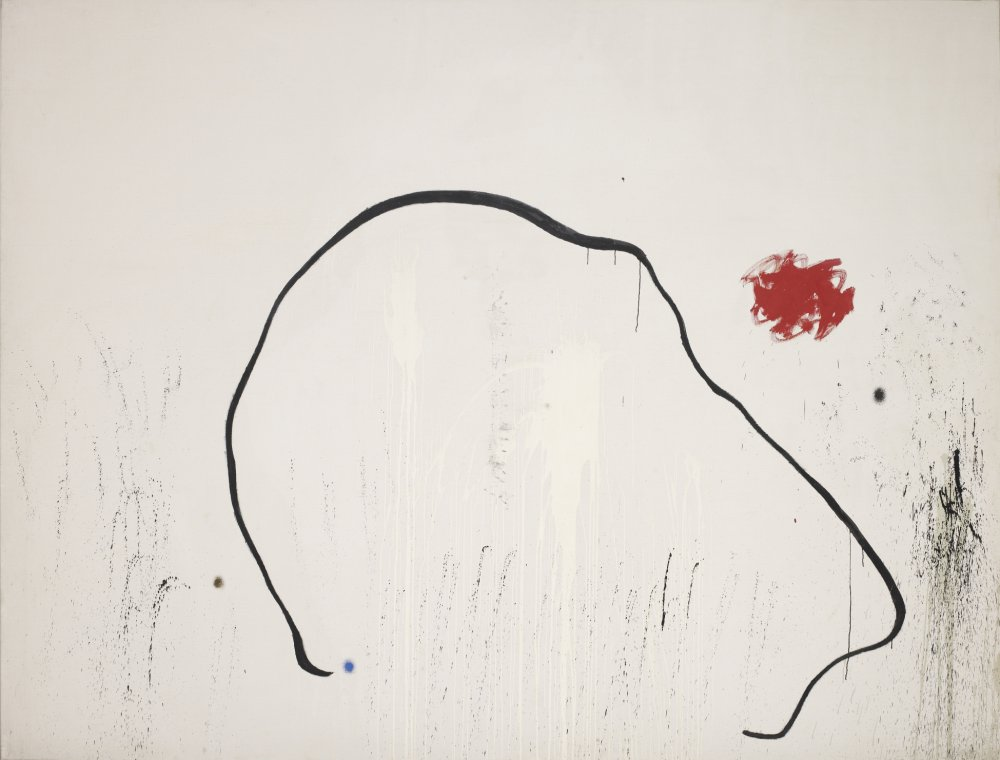
\includegraphics[width=1.8in]{figs/test.jpg} &
%  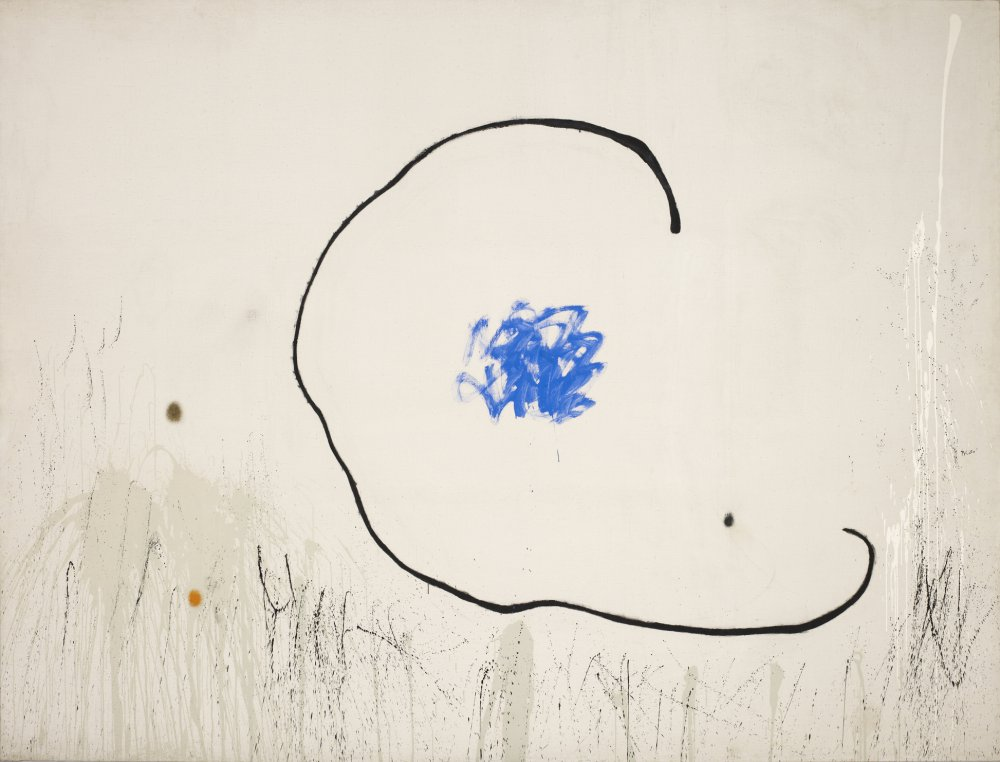
\includegraphics[width=1.8in]{figs/test2.jpg} &
%  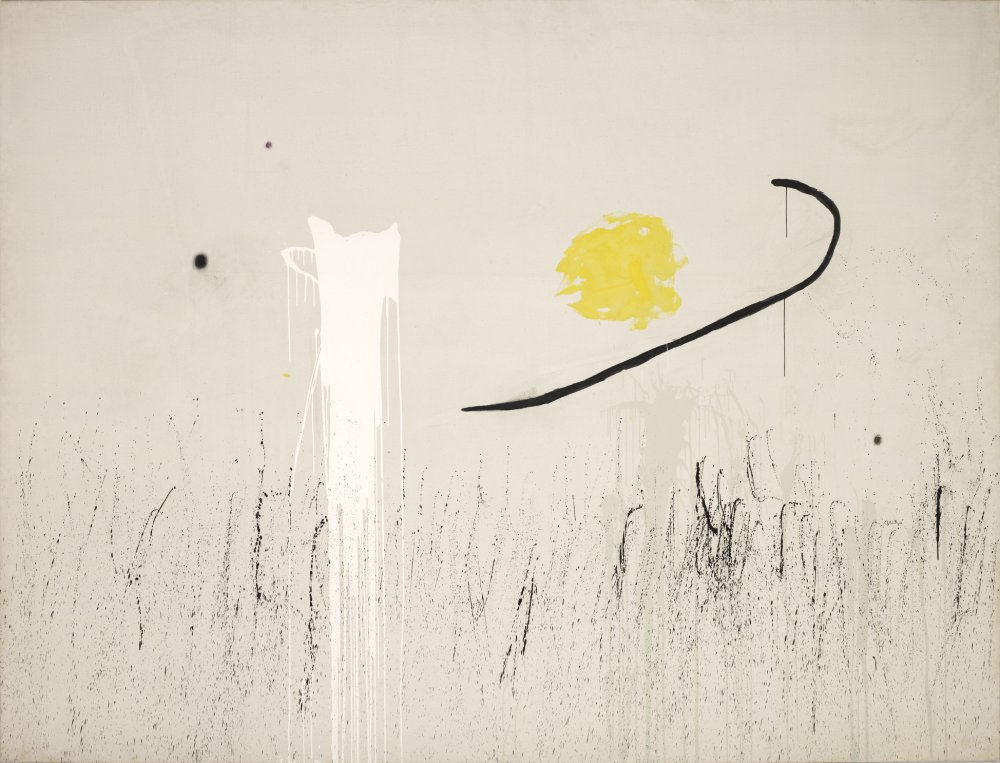
\includegraphics[width=1.8in]{figs/test3.jpg}
%\end{tabular}
%\caption{I-V curve, C-V curve, leakage current vs time. \todo{Temporary picture: Triptic La Esperanza del Condenado, J. Miró}}
%\label{shortslab}
%\end{figure}

\subsection{SKIROC: Silicon pin Kalorimeter Integrated ReadOut Chip}
\label{sec:skiroc}

The SKIROC\cite{Callier:2011zz} (Silicon pin Kalorimeter Integrated ReadOut Chip) is a
very front end ASIC (application-specific integrated circuits)
designed for the readout of the Silicon PIN didoes.
In its version SKIROC2 it consists of 64 channels in AMS 0.35 $\mu$m SiGe technology.
Each channel comprises a low noise charge preamplifier of variable gain followed by two branches:
a fast shaper for the trigger decision and a set of dual gain slow shaper for charge measurement. 
The gain can be controlled by modifying the feedback capacitance during the configuration of the detector.
With the slowest gain, 6pF, the ASIC will handle a linear dynamic range from 0.1 to up to 1500 MIPs 
(a slightly less than the desired final value for the ILC). 
Finally, a Wilkinson type analogue to digital converter fabricates the digitized charge deposition that can be readout. 
Once one channel is triggered, the ASIC reads out all 64 channels adding a bit of information to tag them as
triggered or not triggered and the information is stored in 15 cell deep physical switched capacitor array (SCA).

The SKIROC ASICs can be power-pulsed by taking advantage of the ILC spill structure: 
the bias currents of the ASIC can be switched off during the idle time between bunch trains.
With this method, the ASIC is able to reduce its power consumption down to 25 $\mu$W per channel,
meeting the ILC requirements. All the results shown in this paper are obtained in power pulsing mode.

\begin{figure}[!t]
  \centering
    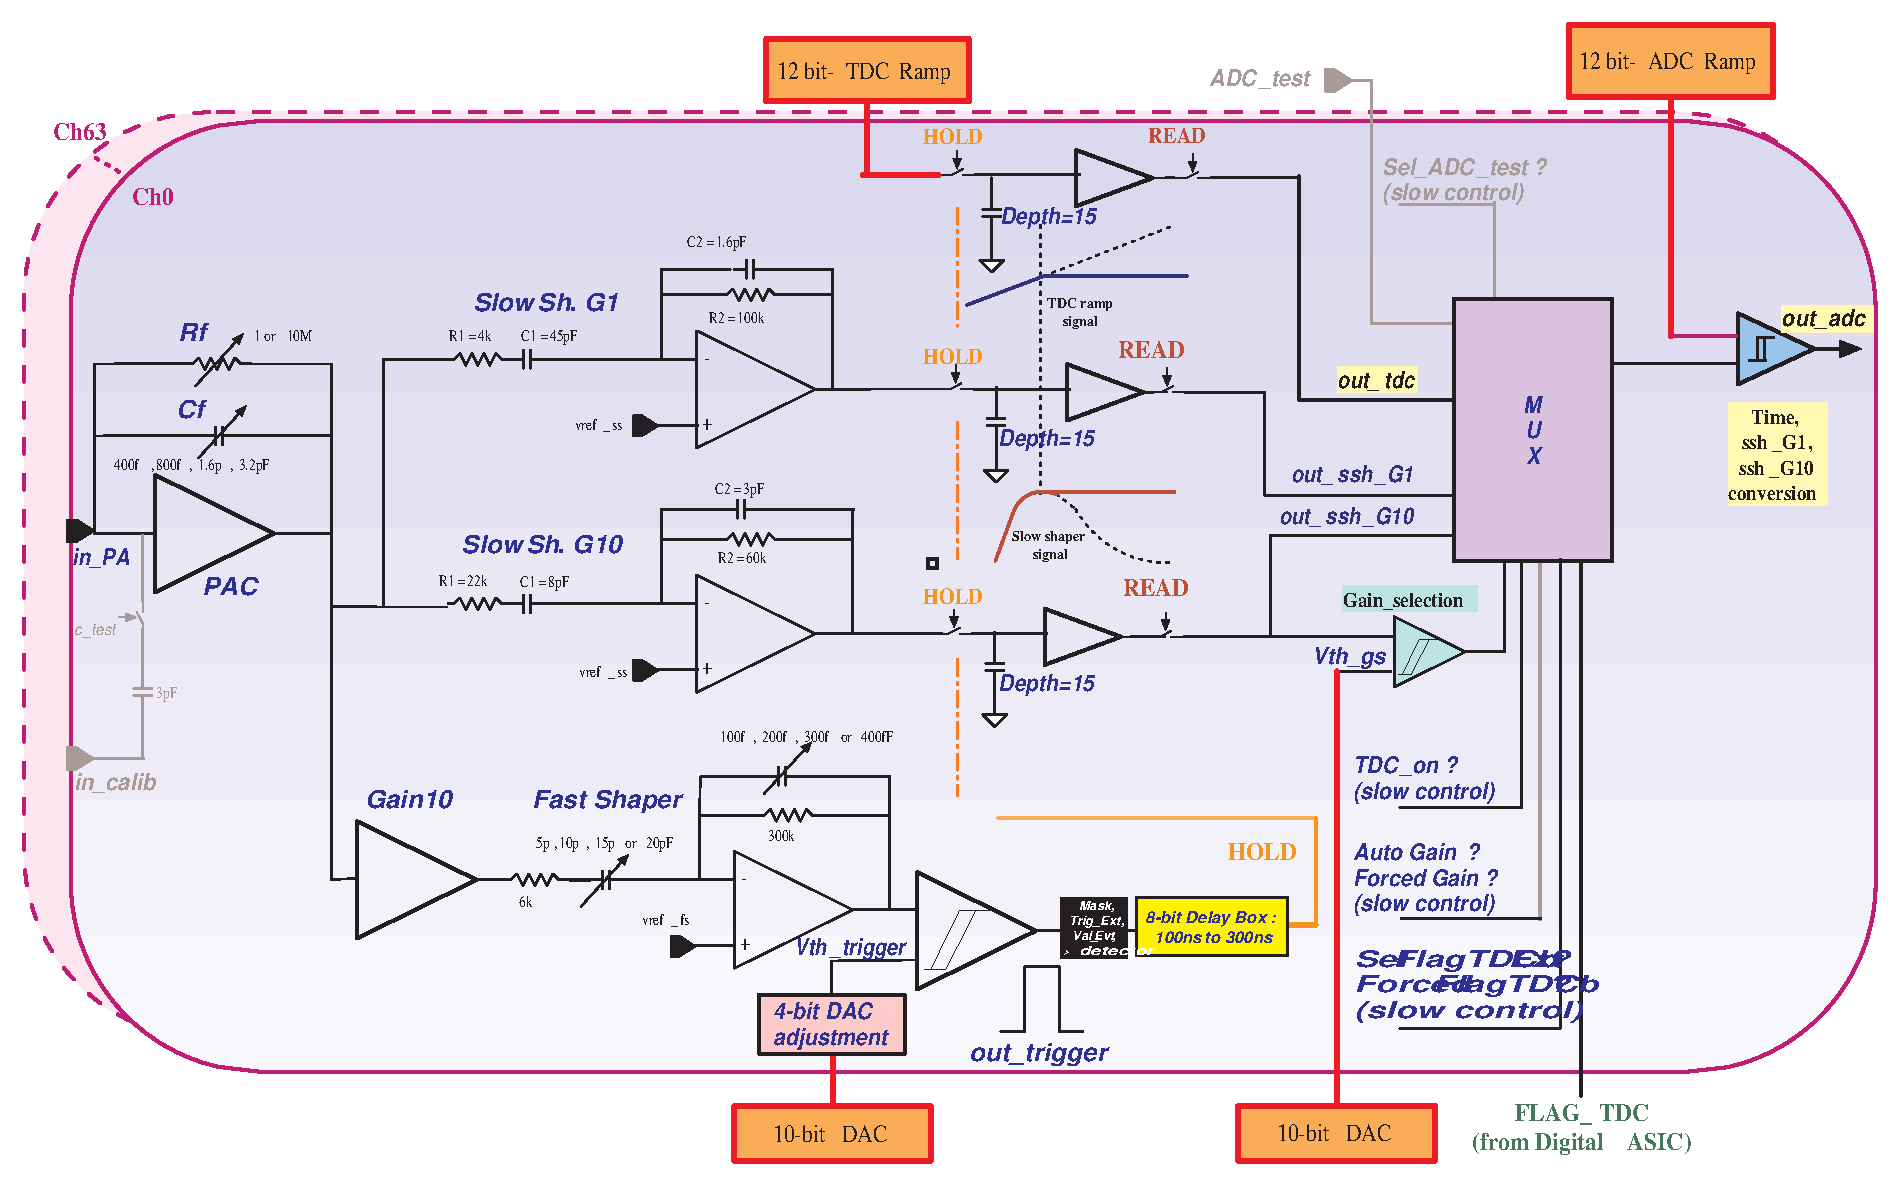
\includegraphics[width=4in]{figs/skiroc2_block.eps}
\caption{The schematics of the analog part of SKIROC2. \todo{High-stack picture (right bottom corner)}}
\label{SKIROC2}
\end{figure}

\subsection{Active Sensor Units}
\label{sec:ASU}

\begin{figure}[!t]
  \centering
  \begin{tabular}{l}
    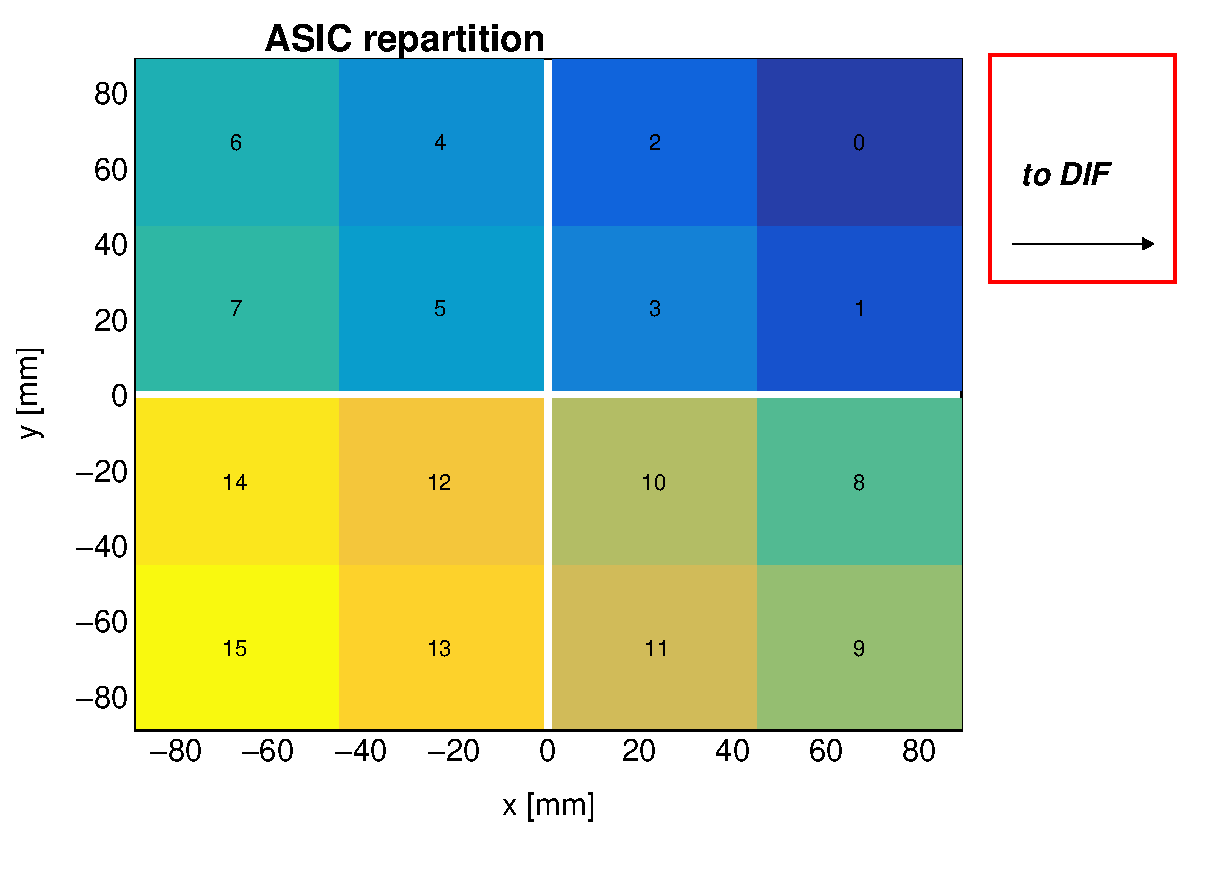
\includegraphics[width=4in]{figs/ASU_geometry1.eps}  \\
    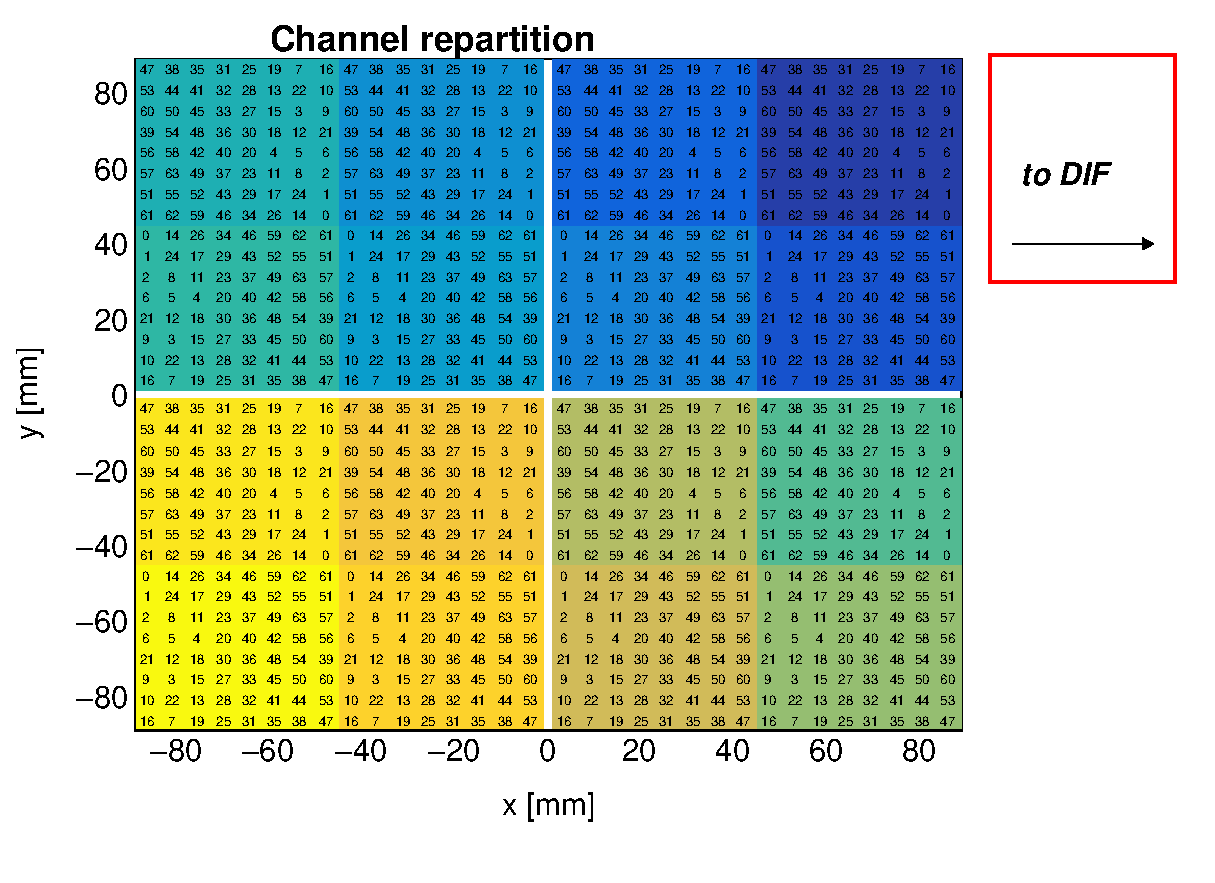
\includegraphics[width=4in]{figs/ASU_geometry2.eps}  \\
  \end{tabular}
  \caption{Repartition of the ASIC (up) and channels (down) in one ASU. In this perspective, the Si-Sensors are in glued in the back.
    The channels are separated (in x and y) by 5.5 mm.
    The empty cross in the middle of the ASU corresponds to the 1 mm separation between the sensors.
    The areas covered by the different ASICs and channels
    are labeled with numbers following design and DAQ criteria: from 0-16 in the case of the ASICs and from 0-63 in the case of the channels.
  }
\label{ASU}
\end{figure}

The entity
of sensors, thin PCB (printed circuit boards) and ASICs is called Active Signal Units or ASU.
An individual ASU has a lateral dimension of 18x18 cm$^{2}$.
The ASUs are currently equipped
further with 16 SKIROC2 ASICs for the read out and features 1024 square pads (64 per ASIC) of 5x5 mm.
The channels and ASICs are distributed along the ASU as shown in Figure \ref{ASU}. Each ASU is equipped with 4 silicon wafers as the described in Section \ref{sec:wafers}.
The high voltage is delivered to the wafers using a HV-kapton sheet that covers the full extension of the wafers.

\subsection{Data AcQuisition system}
\label{sec:DAQ}

The subsequent chain of the data acquisition (DAQ)\cite{Gastaldi:2014vaa} system is inspired by the ILC.
It consists on three modules.
The first module is the so called detector interface (DIF) which is placed at the beginning of each layer holding up to 15 ASUs;
All DIFs are connected by single HDMI cables to the concentrator cards that make
the second module: the Gigabit Concentrator Cards (GDCCs).
%The HDMI connection is used to transmit both slow control and data readout.
This cards are used to control up to 7 DIFs collecting all data from them and distributing among them the system clock and fast commands.
The last module, the most downstream, is the clock and control card (CCC) which
provides a clock, control fan-out of up to 8 GDCCs and accepts and distributes external signals (i.e. signals
generated external pulse generator to simulate the ILC spill conditions).
The whole system is controlled by the Calicoes and the Pyrame DAQ software version 3~\cite{Rubio-Roy:2017ere,Magniette:2018wdz}.
%The Pyrame framework provides basic blocks (called modules) of control-command or data acquisition.
%Calicoes is specific the implementation of these blocks for control-command and data acquisition of the SiW-ECAL prototype. 
%This new version of the DAQ software implements a new mechanism to allow any module to treat and publish data in real time. 
%Those data are made available to any requesting module, in particular to a new online monitor module developed
%for this beam test, allowing for quick online checks of the data quality and integrity.

\subsection{Readout layers and SLABs}
\label{sec:setup}

\begin{figure}[!t]
  \centering
    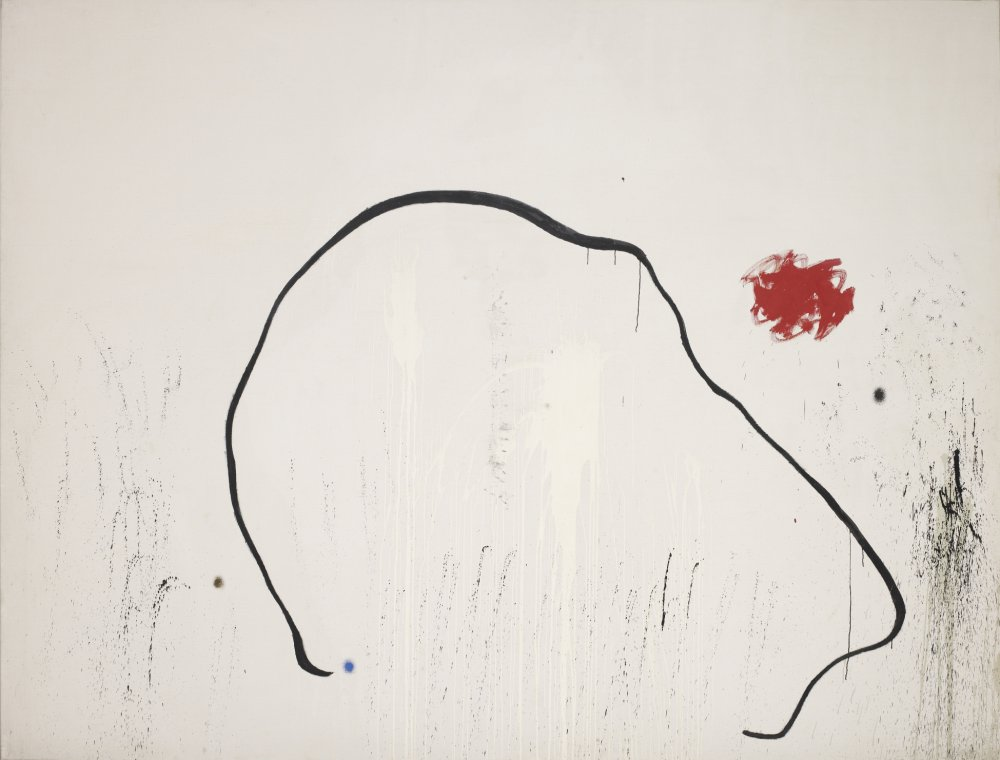
\includegraphics[width=2.8in]{figs/test.jpg} 
  \caption{\todo{Temporary picture: La Esperanza del Condenado, J. Miró}: Open single SLAB with FEV11 ASU, 16 SKIROC 2, interface card and DIF visibles. }
\label{ASU2}
\end{figure}

The readout layers of the SiW-ECAL consist of a chain of ASUs and an adapter board
to a data acquisition system (DAQ) at the beginning of the layer.
This adapter board is called SMBv4
and it also serves as to hold other services as power connectors or the super capacitances used for the power pulsing. 
These capacitances of 400mF with 16 m$\Omega$ of equivalent serial resistance. 
The purpose of these capacitances is to provide local storage 
of the necessary charge to avoid the transport of current pulses over long cables, 
ensuring in this way the stability of the ASICs during the acquisition.

The readout layers are embedded on a "U" shape carbon structure to protect the wafers.
The full system is then covered by two aluminum plates
to provide electromagnetic shielding and mechanical stability.
This ensemble is denominated SLAB
(``short'' for 1 ASU ensembles or ``long'' for several ASUs enchained) and it can be seen in
Figure \ref{ASU2}.
With current SLABs, a potential density of
4000 channels/dm$^{3}$ is achievable. This number should be compared with
the density achieved for previous beam tests: 1500 channels/dm$^{3}$ \cite{Amjad:2014tha}.

\begin{figure}[!t]
\centering
\begin{tabular}{l}
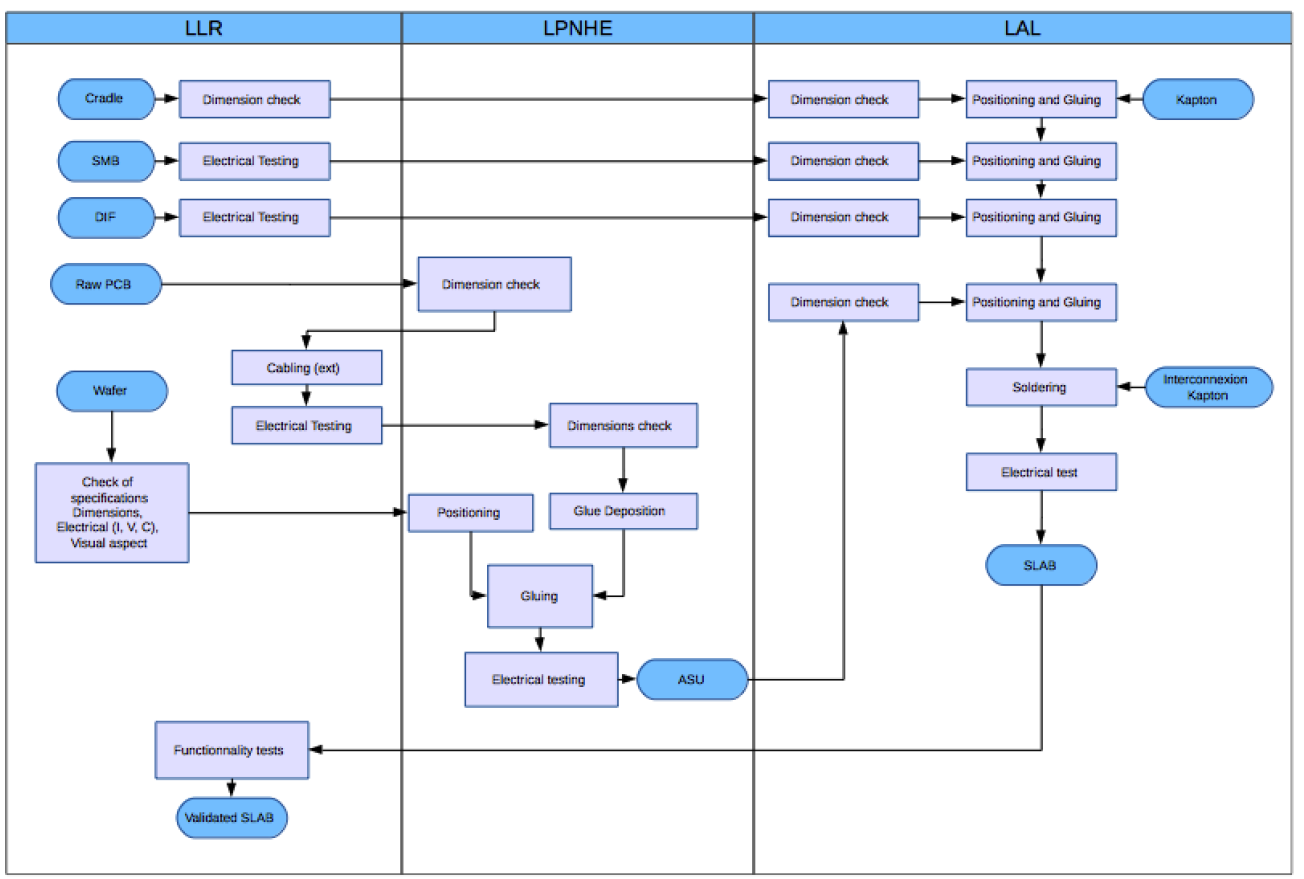
\includegraphics[width=6.0in]{figs/assembly.png} 
\end{tabular}
\caption{Process flow for the assembly of the SiW-ECAL SLABs.}
\label{assembly}
\end{figure}

The SiW-ECAL detector designed for the ILD requires of the order
of $10^{5}$ highly integrated detection like the ones described in this text.
For the production of the small sample of SLABs studied in this document,
a scalable working procedure has been established among several groups \cite{Boudry:2318814}
profiting from the funding of projects like AIDA2020 or the HIGHTEC emblematic project
of the P2IO. A schematic view of this assembly procedure chain can be seen in
Figure \ref{assembly}. For more details we refer to Ref.\cite{Boudry:2318814}.



\section{Commissioning}
\label{sec:commissioning}

This beam test was prepared by a careful and comprehensive commissioning comprising
the debug of the
short SLABSs with special emphasis in the control of the noise and the study of the
prototype performance in cosmic rays tests.

Earlier experiences with the SKIROC2 ASIC are reported in Refs. \cite{Amjad:2014tha,Suehara:2018mqk}). 
Internal SKIROC2 parameters found in these references are adopted in the following
except if the opposite is stated.
For example, the gain value of 1.2pF for the preamplifier is used. 
With this gain, the SKIROC2 ensures a linearity better than 90\% 
for 0.5-200 MIPs, which is enough for 
electromagnetic showers created by few GeV 
electrons or positrons.
% The delay of the trigger signal is the same than in 
%reference \cite{Amjad:2014tha,Suehara:2018mqk}: 130 DAC for all ASICS. 
%This value was chosen by selecting the delay in which an injected signal
%of few MIPs of value get the maximum value of ADC. %Finally, the value of the
%compensation capacitance at the output of the preamplifier has been set to 6pF instead of 
%4pF to prevent overshots and ripples of the signal used as input to the trigger
%decision and ADC lines. 


\subsection{Optimization of noise levels}
\label{sec:comm_noise}

%The purpose of this phase was to monitor and control the
%noise levels of the prototype.
%The commissioning includes the definition of trigger threshold values and a list of noisy channels to be masked.
Studying and control the noise levels
is crucial since noisy channels may saturate the DAQ faster than physical signals.
Two different types of noise sources were identified:
a set of noisy channels randomly distributed in time 
and noise bursts affecting to all layers at the same time.
The outcome of this commissioning is summarized in Figure \ref{noisycells}.

The first type of noise source, noise events randomly distributed in time,
forced us to define a list of channels to be masked in all 
layers. Again, two different type of noisy channels have been identified. 
The first group is compose by randomly distributed in space channels.
The second group is made of
a fixed list of channels, all in the same positions for all SLABs,
and all associated to a higher rate of events with underflowed value
of the read ADC.
%The latter set of channels were identified by means of the online monitoring
%tools.
%As channels are located in the same place for all SLABs,
%we took the conservative assumption
%that all modules would have problems in the same set of channels.
%For example, all channels number 37.
A large amount of these channels are located
in areas of the PCB where the density of lines 
(data and power transmission) is higher than in others.
This hints for an issue on the routing of the PCB.
Therefore, these channels are tagged in Figure \ref{noisycells} with the "routing issues" label
although more tests and deeper inspections of the PCB layout are needed to clarify this issue.

The list of the noisy channels randomly distributed in time and space was
defined by means of dedicated data taking runs. 
These runs were characterized by: their short acquisition windows (open to data recording for 
only 1.1 ms) at low repetition frequencies (5 Hz) to minimize the chances of having real events due to cosmic rays 
hitting the detector during the
data taking; and the relatively high trigger threshold values between 250 and 400 DAC 
(which are equivalent to $\sim$0.5-2 MIP, see Section \ref{sec:comm_trigger} for more 
information). The full process was an iterative process starting with several repetitions
of runs at a high threshold value and then some iterations at lower threshold but always 
higher than 0.5 MIP. 
In each of the iterations, the channels identified as noisy were masked.
A full run involved 3-5 threshold values and at least two repetitions per value.
Again, we decided to follow a conservative approach for list the noisy channels to be masked:
if the channel was triggered at rates larger than 0.5-1\% of the total number of triggers per ASIC
it was added to the list. These channels are labeled as "other" in the first plot in  Figure \ref{noisycells}.

In addition to the different noisy channel types described above, we also have
masked full sectors of the SLABs if an ASIC was faulty (at least 70\% of channels 
listed as noisy) or if a Si-wafer was misworking (high leakage currents). In these cases 
and in all mentioned above, the masking involved two steps: disabling of the trigger and 
the disabling of the power of the preamplifier of that channel.

\begin{figure}[!t]
  \centering
  \begin{tabular}{l}
  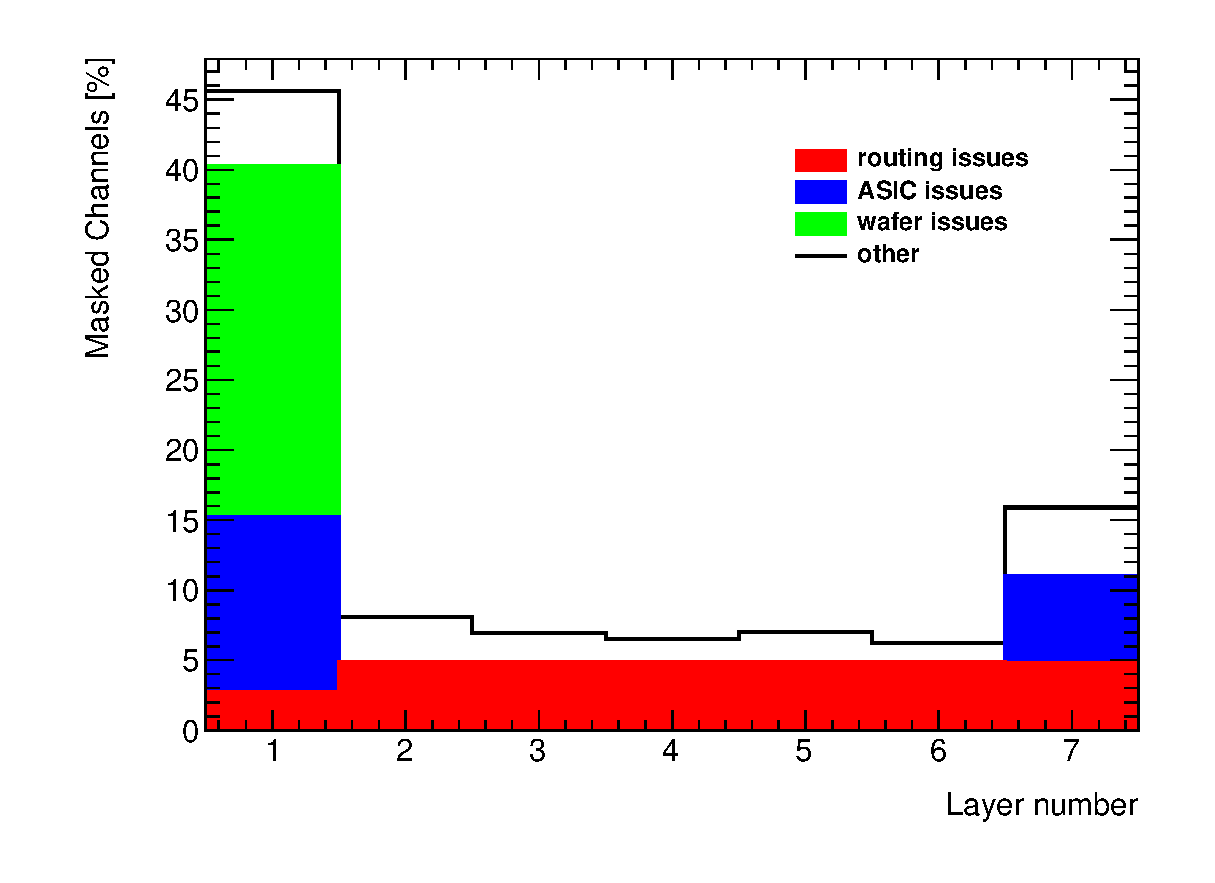
\includegraphics[width=4in]{figs/commissioning/masked_layer.eps} \\
  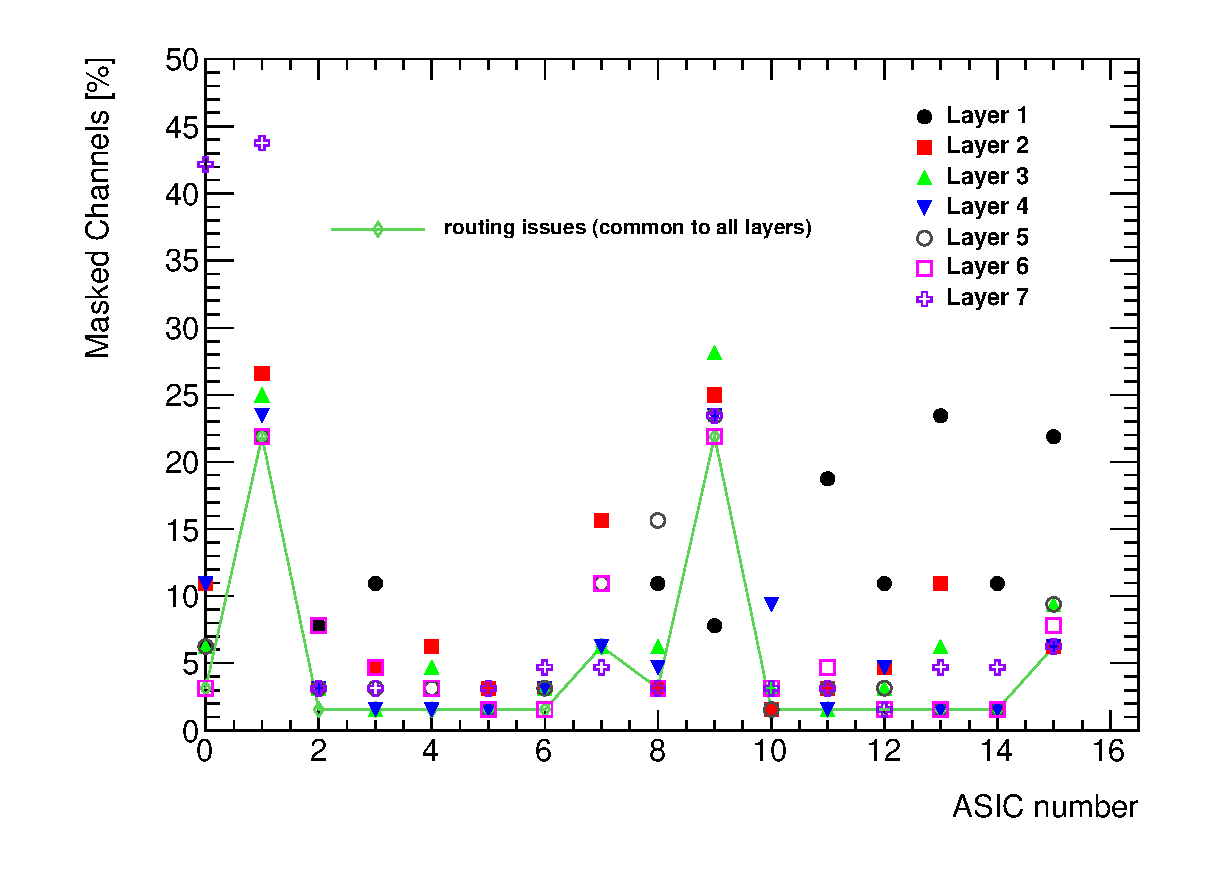
\includegraphics[width=4in]{figs/commissioning/masked_chip.eps}
  \end{tabular}
\caption{Ratio of channels that are marked as noisy in all slabs. 
Top: inventory of the different type of noisy channels per slab. 
Bottom: break down of the total number of noisy channels per ASIC. 
The ASICs 4-7 (wafer issue) and 10 from layer 1 and the ASIC 4 from layer 7 are not included
in the second plot since they are fully masked.}
\label{noisycells}
\end{figure}

The other source of noise mentioned at the beginining of this section
consist on noise bursts happening coherently at the same time in all SLABS
and it was correlated to occasions when the electrical isolation between SLABs was broken.
This is a hint of a system effect as can be the appearance of
grounding loops or disturbances in the power supplies.
The issue was circumvented by improving the electrical isolation of single layers.
We have also observed that the noise bursts happens only at the end of long acquisitions. Therefore, in addition to the improved isolation,
we selected short enough acquisitions windows (which indeed are the most appropriate to the high rates of particles in the DESY beam).
Ddedicated studies in the laboratory are currently pngoingin order to fully understand this issue.

The list of channels mentioned above is discarded from the data taking from now on.

\subsection{Threshold determination}
\label{sec:comm_trigger}

In order to select the optimal trigger threshold values for the detector operation
we perform dedicated scans of trigger threshold values
with all channels enabled (excepted the marked as noisy). 
The threshold values are given in internal DAC units which are translated to
meaningful physical quantities in Section \ref{sec:comm_trigger_sn}. 
The threshold scan curves made of the total number of hits normalized to 1 vs the threshold
for each channel are modeled by a complementary error function called ThS curves from now on:

\begin{equation}
ThS(DAC)=p_{0} \times erfc(\frac{DAC-p_{1}}{p_{2}}) = 
\newline
\frac{2p_{0}}{\sqrt(\pi)} \int_{\frac{DAC-p_{1}}{p_{2}}}^{\infty} e^{-t^{2}} dt,
\label{eq_S-curve}
\end{equation}
where $p_{0}$ is 1/2 of the normalization, $p_{1}$ is the value in which the noise levels are 
the 50\% of its maximum and $p_{2}$ give us the width of the ThS curve. 

In the absence of external signals (cosmic rays, injected signals, etc) 
these noise ThS curves show the convolution of the envelope of the 
electronic noise at the output of the fast shaper (the trigger decision branch on the SKIROC).
Indeed, the size of this envelope is related to the slow clock frequency.

To reduce to the minimum the presence of cosmic rays signals, 
we perform runs with short open acquisition windows
as described in the previous section.
In Figure \ref{scurve_channels} 
two result of two threshold scans and the fit by
a ThS curves for two different channels from the second layer of the setup are shown.

\begin{figure}[!t]
  \centering
  \begin{tabular}{ll}
  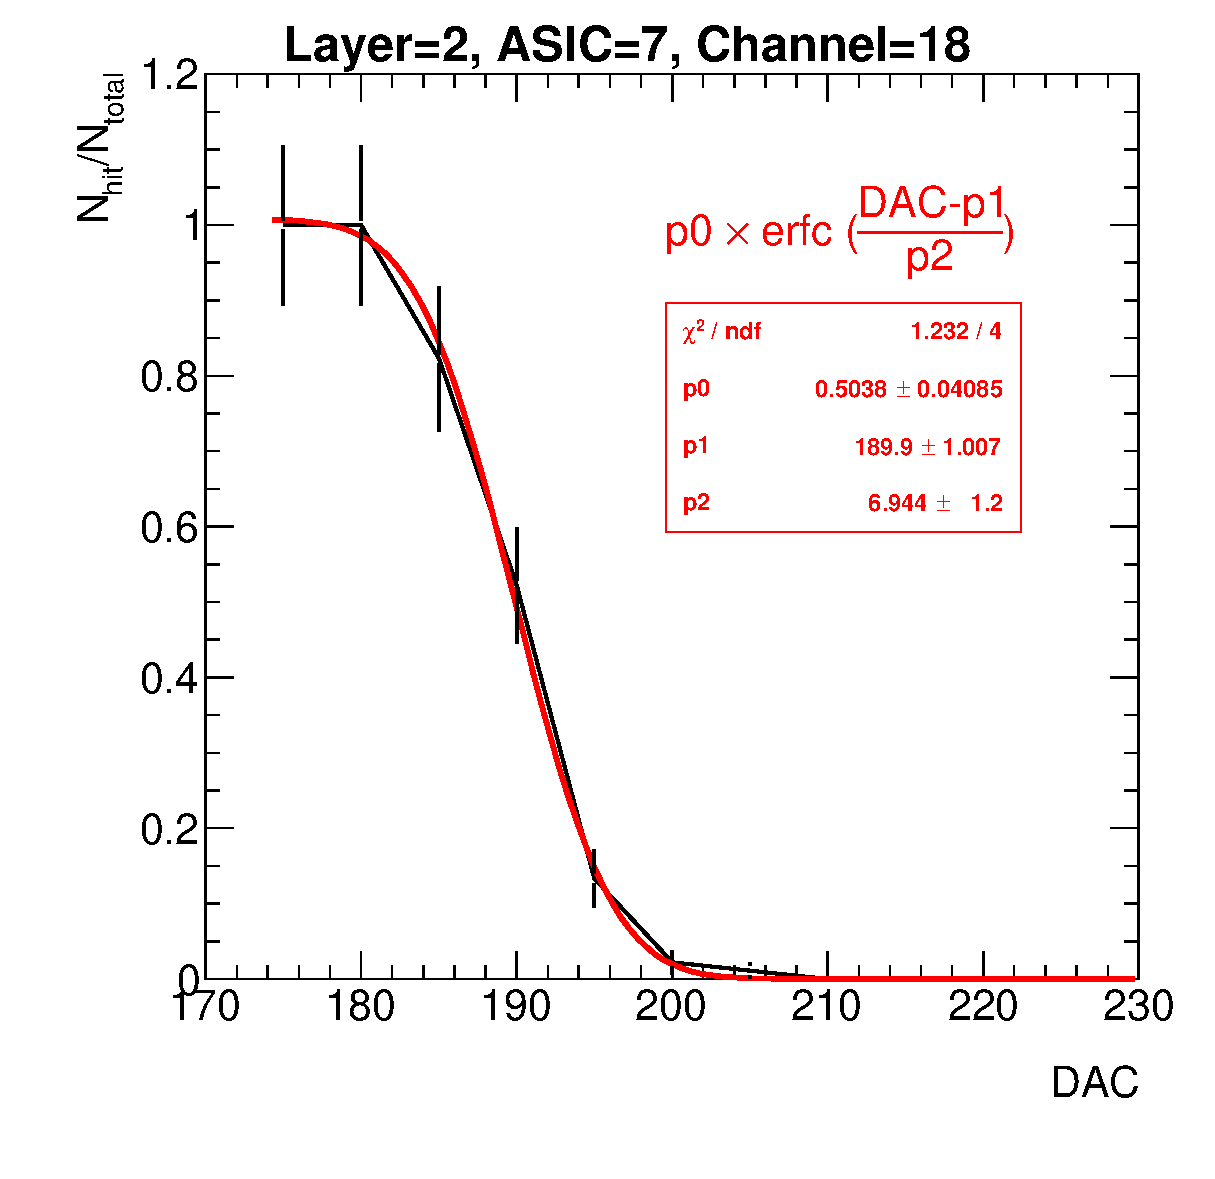
\includegraphics[width=2.8in]{figs/commissioning/scurve_chn18_asic7_layer2.eps} & 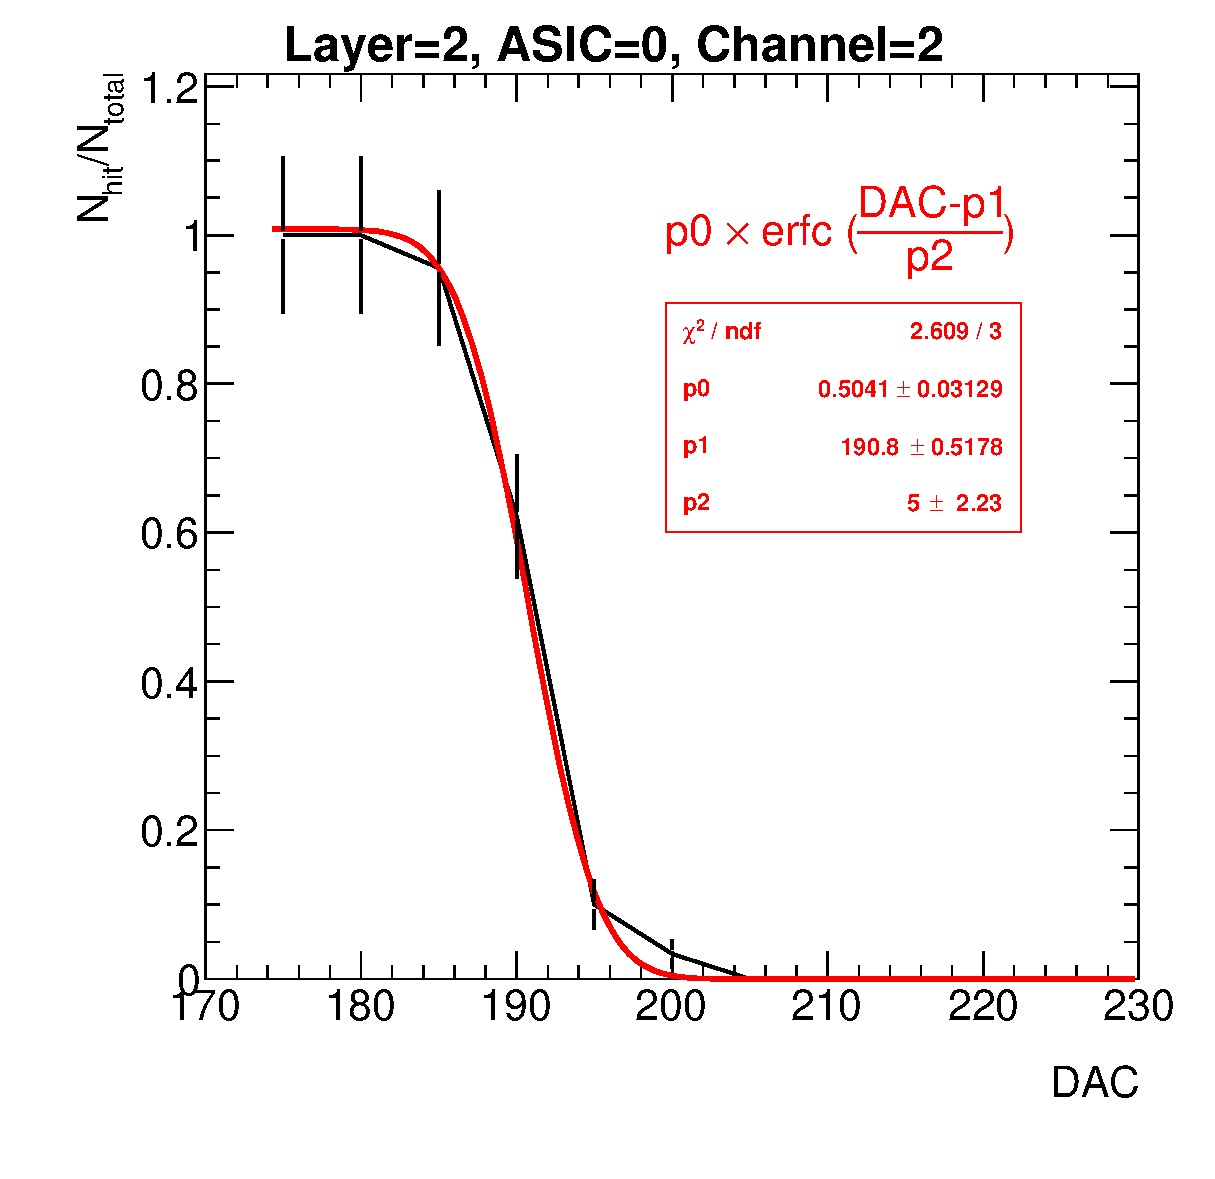
\includegraphics[width=2.8in]{figs/commissioning/scurve_chn2_asic0_layer2.eps}
  \end{tabular}
\caption{Two threshold scan curves and their associated ThS curves.}
\label{scurve_channels}
\end{figure}

The function from equation \ref{eq_S-curve} was fitted to all
channels data and all the values of $p_{1}$ and $p_{2}$ were saved.
The final threshold value of every ASIC, in DAC units, was chosen 
by taking the 

\begin{equation}
maximum(DAC_{optimal}^{ASIC-j} = <p_{1}^{ASIC-j}> + 5 \times <p_{2}^{ASIC-j}>,230)
\end{equation}

if at least the the 30\% of the 64 channels ThS curves in the ASIC could be fitted.
If only less  than the 30\% of curves of the 64 channels were
succesfully fit, a global DAC value of 250 was set.
The $<>$ denotes the average over all the channels on the ASIC.
The choice of these two values was 
sustained by previous experiences, see for example \cite{Amjad:2014tha}.

The optimal trigger threshold values for all ASICs are shown in Figure \ref{trigger_thresholds}.


\subsection{S/N ratio in the trigger line}
\label{sec:comm_trigger_sn}

Similar kind of measurements can be done but using external signals. 
This will allow to calculate the signal over noise (S/N) ratio to trigger 1 MIP signals.
To calculate the S/N of the trigger we need to compare the 1 MIP ThS curve and 2 MIP ThS curve. The S/N 
will be defined as the ratio between the distance of both ThS curves at its 50\% and the width of the 
ThS curve.

In Figure \ref{scurves_injection} we see the 1 MIP and 2 MIP ThS curves obtained for several channel
in a SKIROC testboard in which a single SKIROC2 in BGA package is placed and the 1 MIP and 2 MIPs 
 signals are directly injected in the preamplifier 
(via a 3 pF capacitor located in the injection line as shown in Figure \ref{SKIROC2}). 
From this plot we can extract a S/N ratio of $\sim$12.8. 
We do not expect large differences with the results that we would obtain with 
a full equipped SLABs 
although this board is thought for commissioning and test of the SKIROC ASICS in an
"ideal" environment in contrast with the FEV
ASUS that are optimized to meet the detector requirement and to hold several ASICs at the same time.
%For example: only power pulsing of the analog power is done in this testboard,
%there is a set of external capacitors on the board connected to some ASIC pins and
%usually only one channel is tested. This board allows us to commission and debug the SKIROC itself
%but not the full system.

\begin{figure}[!t]
    \centering
  \begin{tabular}{l}
	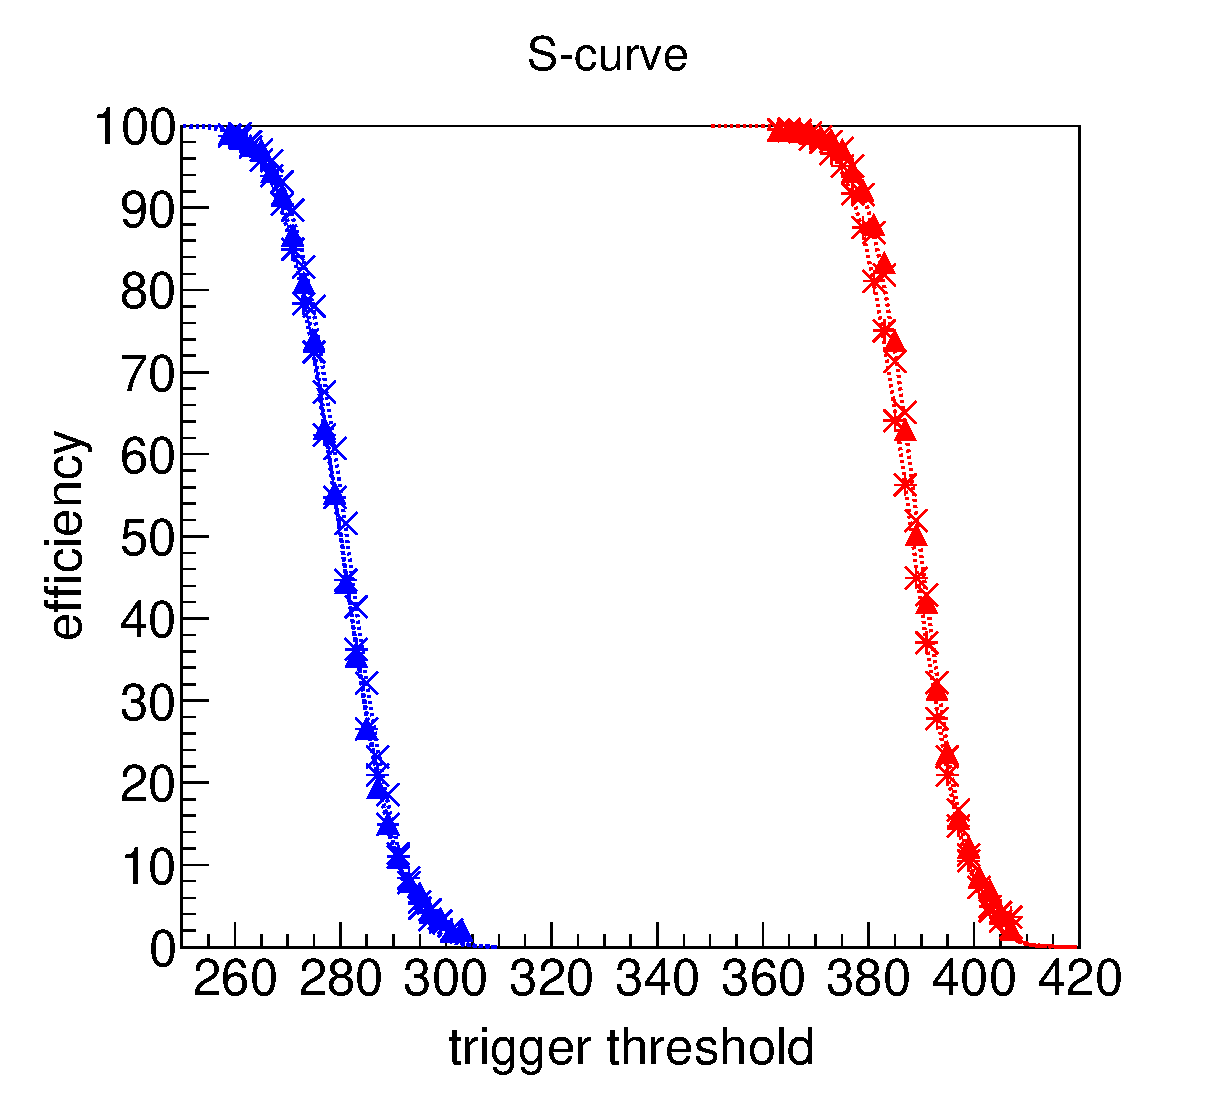
\includegraphics[width=4in]{figs/commissioning/scurve_pp_fastshaper_ch.eps} \\
	\end{tabular}
\caption{ThS curves with charge injection (1 MIP in blue and 2 MIPs in red) for two different channels in a SKIROC2 testboard. From this plot, we extract a $S/N = 12.8$ in the trigger line.}
\label{scurves_injection}
\end{figure}


We have obtained similar results using real signals, in this case cosmic rays signals by using very long
acquisition windows of 150 ms at 5 Hz. This is shown 
in Figure \ref{scurves_cosmics}  where 
we show the result of the fit to the noise ThS curves for all channels individually (in red) in one of the ASICs of 
the second layer together with the results of the ThS curve obtained with cosmic rays integrated for all channels
(black points and blue line).
%For the cosmic ThS curve we took 30 min of data per point using very long spills (150 ms) in 
%frequencies of 5Hz and we add up the triggers from all channels together. In addition, using the 
%knowledge of the MIP value (see next section), we performed a simple cut in the ADC
%to keep only signals corresponding to a MIP 
%(pedestal subtracted) $\pm30$ ADC counts. With this cut we try reduce the contribution of muons 
%traversing the wafers with very large angles but we don't have a way to select perpendicular tracks 
%since we were using simple setups with only single slabs. 
We expect
a broader distribution of the cosmic ThS curve since muons can traverse
the detector at different incidence angles.  
In addition to this, we should remember that the noise ThS curve do correspond to the real noise 
distribution but only to the envelope of the noise in the fast shaper, therefore the
distance between the two ThS curves is smaller than the real distance between noise and signal.
Therefore, if we calculate the S/N 
using this plot, the value would be unrealistic but at least provides 
the comparison between the ThS curve for 1 MIP real and injected signals.

\begin{figure}[!t]
    \centering
  \begin{tabular}{l}
	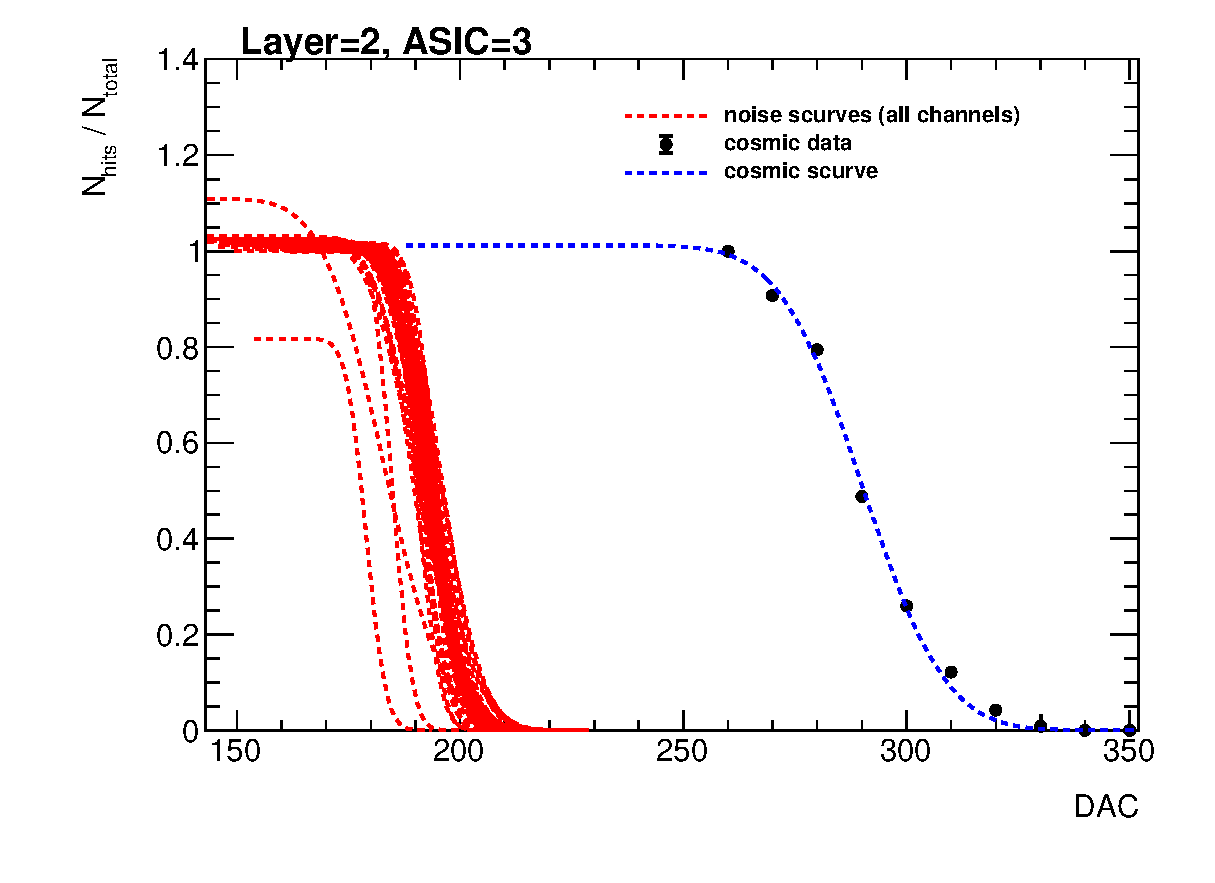
\includegraphics[width=4in]{figs/commissioning/cosmic_scurves_asic3_layer2.eps} 
	\end{tabular}
\caption{ThS curves for noise (channel by channel, only the result of the fit) and cosmic rays (all channels together) for one ASIC in layer 2.}
\label{scurves_cosmics}
\end{figure}

Both ways of estimating the S/N ratio of the trigger have their own limitations
and dedicted studies in beam test are needed in order to
precisely determine it.
In the meanwhile, combining the information contained in the Figs \ref{scurves_injection} and \ref{scurves_cosmics},
we can estimate the value in energy at wich we have set our trigger threshold.
This is shown in Figure \ref{trigger_thresholds}.% Two ASICS have a
%trigger threshold value of 0.67 MIP. The 11\% of the ASICs have a trigger threshold between 0.5 and 0.55 MIP and the rest, 87\%, have trigger thresholds slightly lower 0.5 MIP.

\begin{figure}[!t]
  \centering
  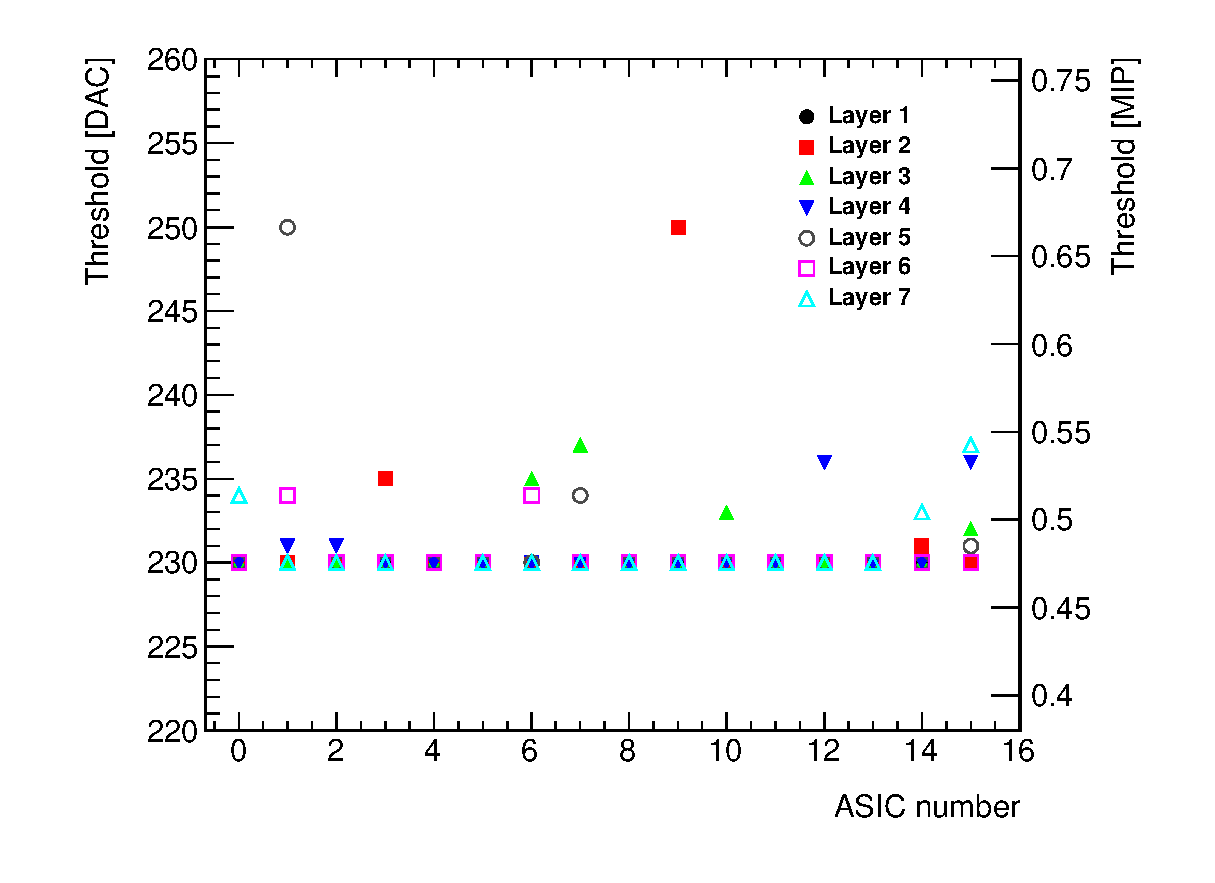
\includegraphics[width=4in]{figs/commissioning/threshold_chip.eps}
  \caption{Summary of the trigger threshold settings in internal DAC units and in MIP units.}
\label{trigger_thresholds}
\end{figure}


\subsection{Prospects}
\label{sec:comm_prospects}

All the commissioning procedure described above relies in very conservative decisions
due to the presence of unknown noise sources during most of the commissioning phase. These sources are
now well know and isolated and therefore a new ``noise commissioning procedure'' has been studied.
It will consist in an iterative algorithm that first
will identify and mask the channels giving underflowed signals and afterwards run a set of acquisitions
in which the number of triggers per channel will be compared with the number of expected triggers
assuming only cosmic rays as signal. This will allow us to have an
unambiguous definition of the noise levels channel per channel instead of 
defining such levels relatively to the total number
of recorded triggers per ASIC. Finally, once that the noisy channels
are identified, the optimization of the threshold levels
will be performed and a last run for identification of noisy channels will be taken using this optimal
threshold.
%In this run, we can decide to mask the noisy channels or
%to increase its own trigger threshold level if we are using Skiroc2a.

Using this new procedure we manage to reduce the number of masked channels by a factor 2 without any loss of performance,
at least in the laboratory and using 3 of the 7 SLABs. This new procedure will be tested in the next beam test.
Also, in order to
optimize the commissioning of the detector,
we propose a new set of measurements in the next beam test such as
a scan of optimal delay of the hold values of the trigger using MIP like particles
and a threshold scan for the determination of the S/N in the trigger line. This later
can be done by the comparison of ThS curves taken with 1 MIP and $\sqrt{2}$ MIP signals (tilting the detector by 45 degrees).


\section{Performance on positron beam test at DESY}
\label{sec:beamtest}


The beam test line at DESY provides continuous positron beams in the energy range of 1 to 6 GeV with
rates from few hundreds of Hz to few KHz with a maximum of $\sim 3$ KHz for 2-3 GeV. 
The particles beam ies produced as follows: first, the electron/positron synchrotron DORIS II 
is used to produced a photon beam via bremsstralhung when interacting with a carbon fiber target;
secondly, these photons are then converted to electron/positron pairs; 
and, finally, the beam energy is selected with dipole magnets and collimators. 
In addition, DESY gives acces to a bore 1 T solenoid, the PCMag.

\begin{figure}[!t]
\centering
\begin{tabular}{l}
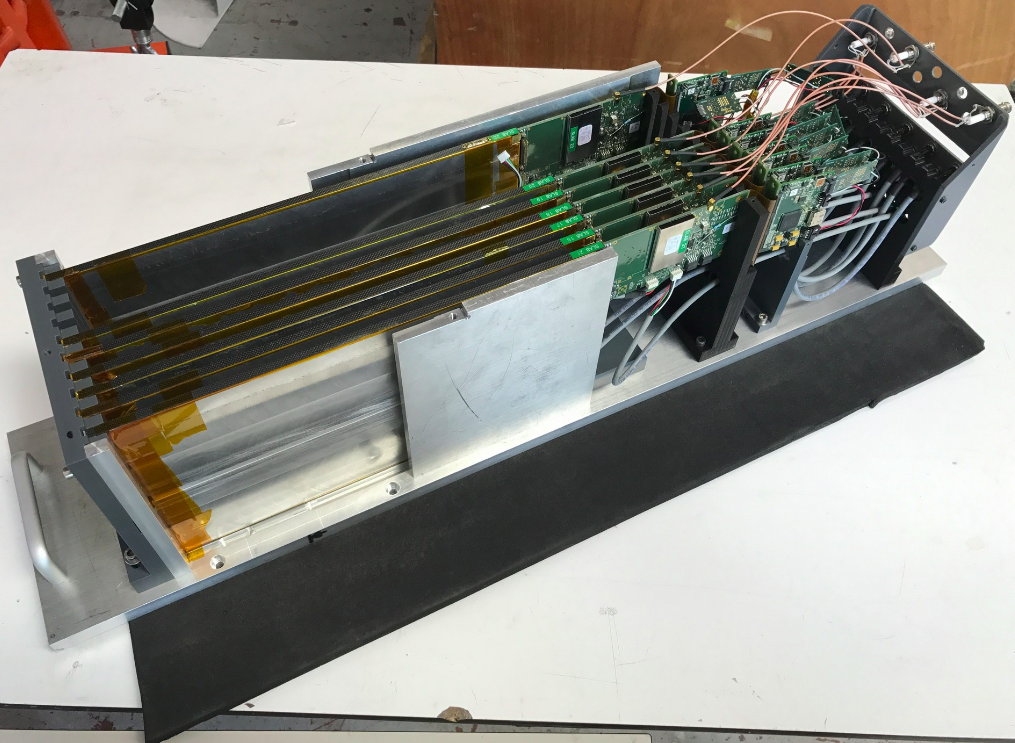
\includegraphics[width=4.0in]{figs/proto.png} 
\end{tabular}
\caption{Prototype with 7 layers inside the aluminum stack.}
\label{proto}
\end{figure}

A photograph showing the SiW-ECAL technollogical prototype setup can be seen in Figure \ref{proto}.
Current prototype consists on 7 layers of SLABs housed by a PVC and aluminum structure that can hold up to 10.
For the beam test described in Section \ref{sec:beamtest} all the layers were separated by equal distances of 15 mm
except the last one which was at 60 mm of its nearest. In the following sections, we will refer to layers number 1 to 7, where
the 1 is the closest to the beam pipe and 7 is the farthest.
The detector was exposed to a positron beam in the DESY test beam area (line 24).
By means of an external pulse generator we defined the length of the acquisition window to be
3.7 ms at a frequency of 5 Hz.
The detector was running in power pulsing mode without any extra active cooling system.

The physics program of the beam test can be summarized in the following points:

\begin{enumerate}
\item Calibration without tungsten absorber using 3 GeV positrons acting as minimum ionizing particle (MIPs) directed to 81 position equally distributed over the modules.
\item Test in magnetic field up to 1 T using the PCMag. For this test a special PVC structure was
designed and produced to support one single SLAB.	
The purpose of such test was twofold: first to prove that the DAQ, all electronic devices and the 
mechanical consistency of the SLAB itself are able
to handle strong magnetic fields; 
second to check the quality of the data and the performance of the detector during the data taking when running
in a magnetic field.
\item Response to electrons of different energies with fully equipped detector, i.e. sensitive parts {\it and} W absorber, with three different repartitions of the absorber material:
\begin{itemize}
\item W-configuration 1: $0.6,1.2,1.8,2.4,3.6,4.8$ and $6.6~X_{0}$
\item W-configuration 2: $1.2,1.8,2.4,3.6,4.8,6.6$ and $8.4~X_{0}$
\item W-configuration 3: $1.8,2.4,3.6,4.8,6.6,8.4$ and $10.2~X_{0}$
\end{itemize}
\end{enumerate}

First reports on this beam test can be find in
Refs. \cite{Irles:2018uum,Irles:2018hcd}. In this paper we discuss in more detail
the results of the pedestal, noise and MIP calibration in Section \ref{sec:calib}.
We show also results on the pedestal and noise stability when running inside
a magnetic field in Section \ref{sec:magnet}. Finally, a first peek to the 
response and stability of the detector in electromagnetic showers events is discussed in 
Section \ref{sec:showers}. 

\subsection{Response to MIP-acting positrons}
\label{sec:calib}

\subsubsection{Pedestal and noise determination}
\label{sec:pedestal}

The calibration runs have been used to calculate the pedestal distribution reference values 
and the noise levels (the width of the pedestal distrution) of each channel.
In Figure \ref{signal_pedestal} we show the signal and pedestal distribution of a single channel after
subtracting the pedestal mean position. The results of the MIP calibration fit are included (red) and explained in the next version.
The pedestal distribution is shown only for the first SCA to keep the y-axis within a reasonable range.
The signal distribution is integrated over all SCAs.

\begin{figure}[!t]
  \centering
  \begin{tabular}{l}
    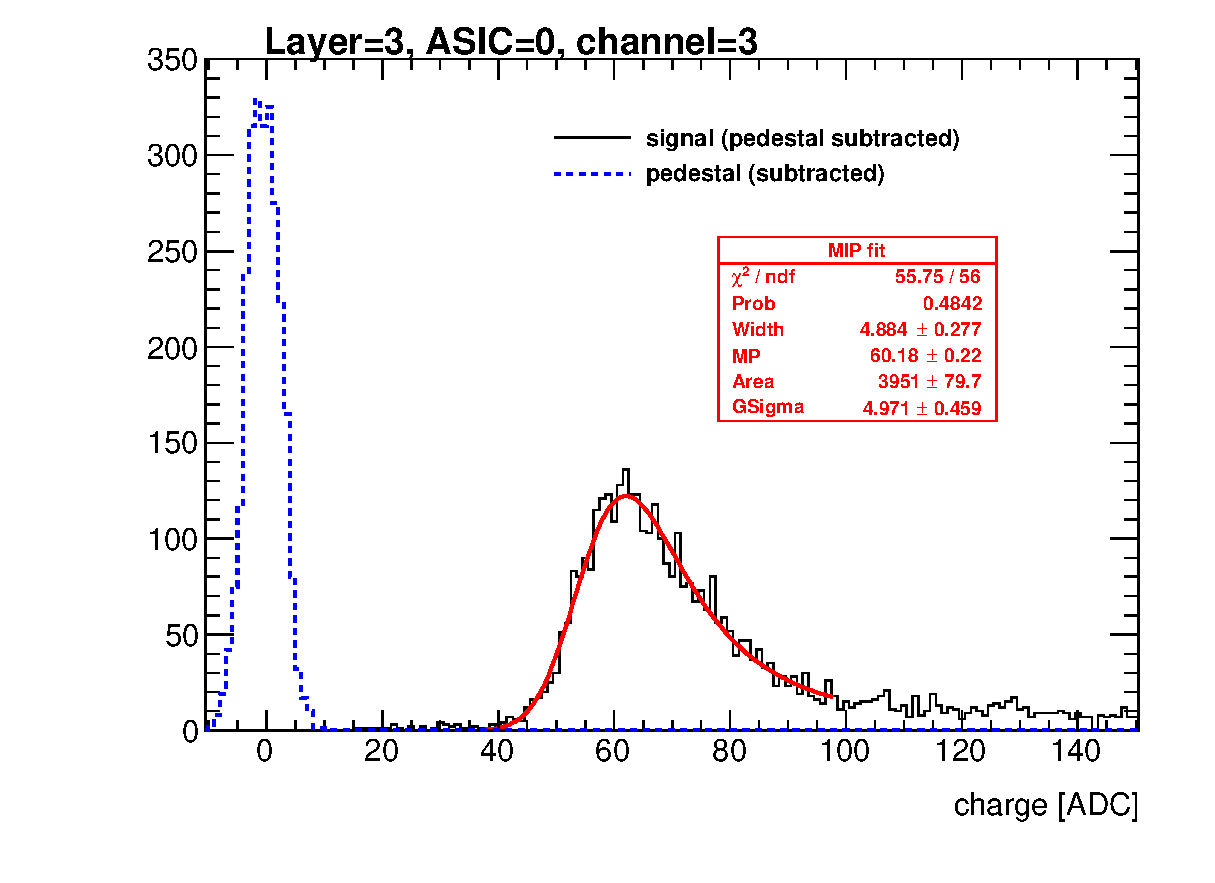
\includegraphics[width=4in]{figs/mip_pedestal_example.eps}
  \end{tabular}
  \caption{Pedestal (blue dashed line) and signal (black continuous line) distribution for one channel in the third layer.}
\label{signal_pedestal}
\end{figure}

The pedestal is calculated as the mean position of
the ADC distribution of channels without trigger. The noise is
associated to the width of such distribution.
The pedestal correction is done layer-, chip-, channel- and SCA-wisely due to the large spread of values between pedestals, as observed in 
Figure \ref{pedestal_layer} (left plot) and Figure \ref{pedestal_all} (also left plot).
For the noise, the dispersion is much smaller ($\sim 5 \%$). This is shown in the right plots of Figures \ref{pedestal_layer} and \ref{pedestal_all}.
From now on, the pedestal correction is applied to all the results presented.

%\begin{figure}[!t]
%  \centering
%  \begin{tabular}{ll}
%    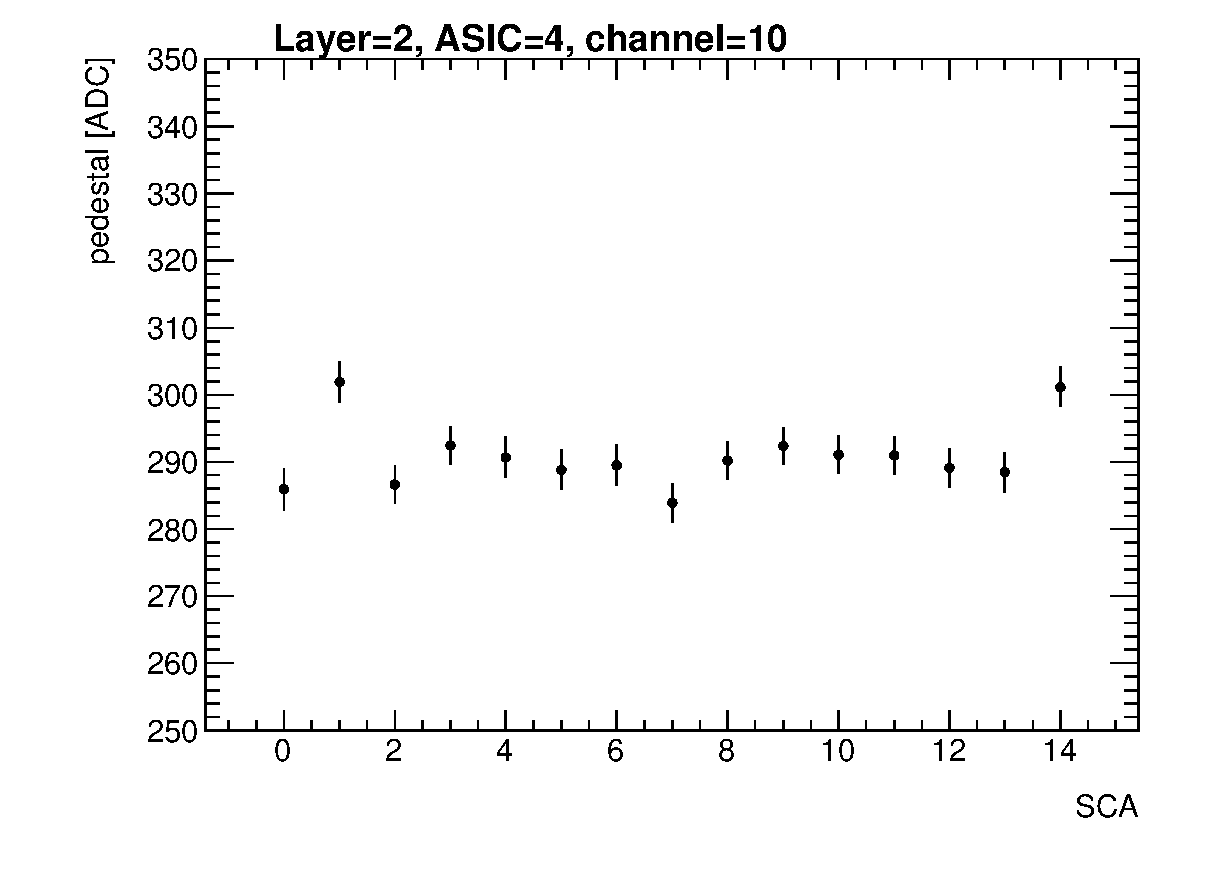
\includegraphics[width=2.8in]{figs/pedestal/ped_mean_layer2_chip4_cell10.eps} & 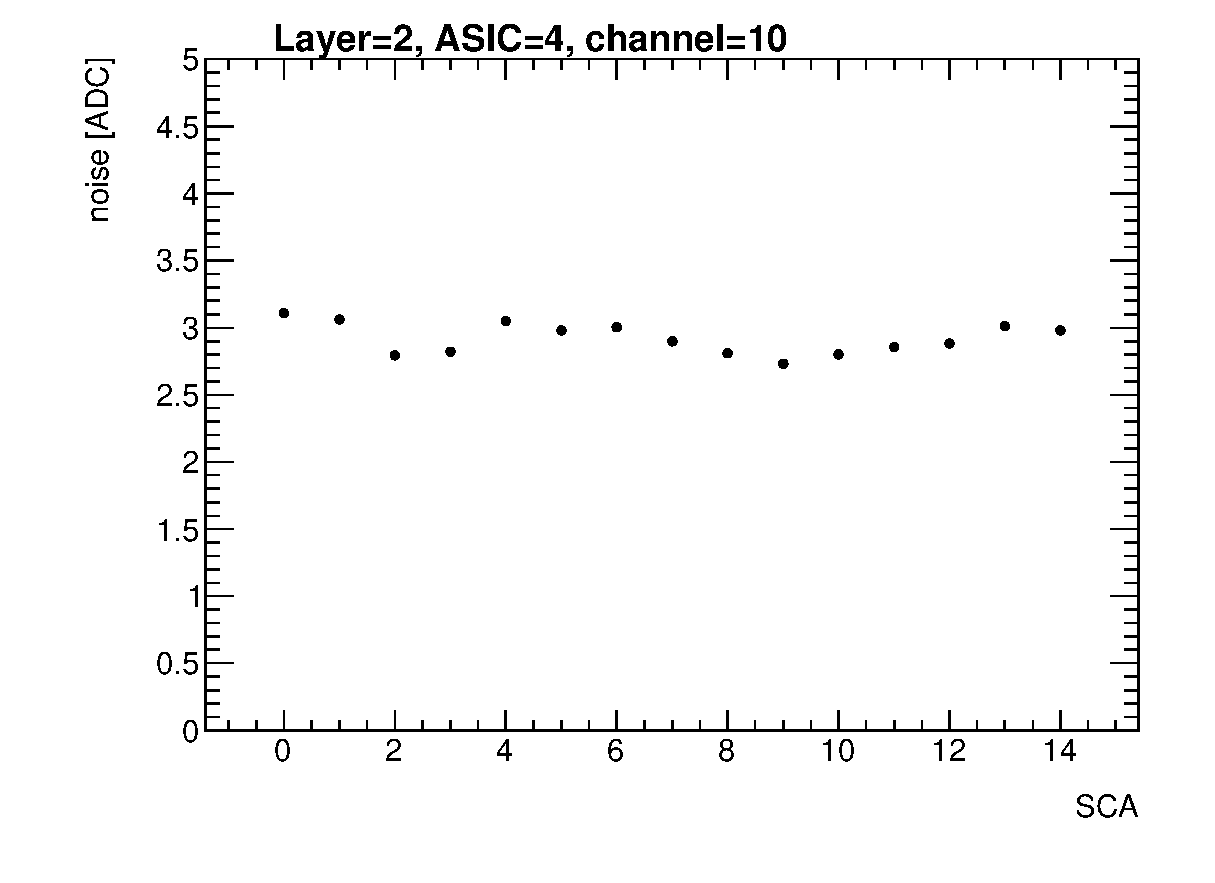
\includegraphics[width=2.8in]{figs/pedestal/ped_width_layer2_chip4_cell10.eps}
%  \end{tabular}
%  \caption{Pedestal mean position (left) and width (right) for one channel in the second layer.}
%\label{pedestal_channel}
%\end{figure}

\begin{figure}[!t]
  \centering
  \begin{tabular}{ll}
    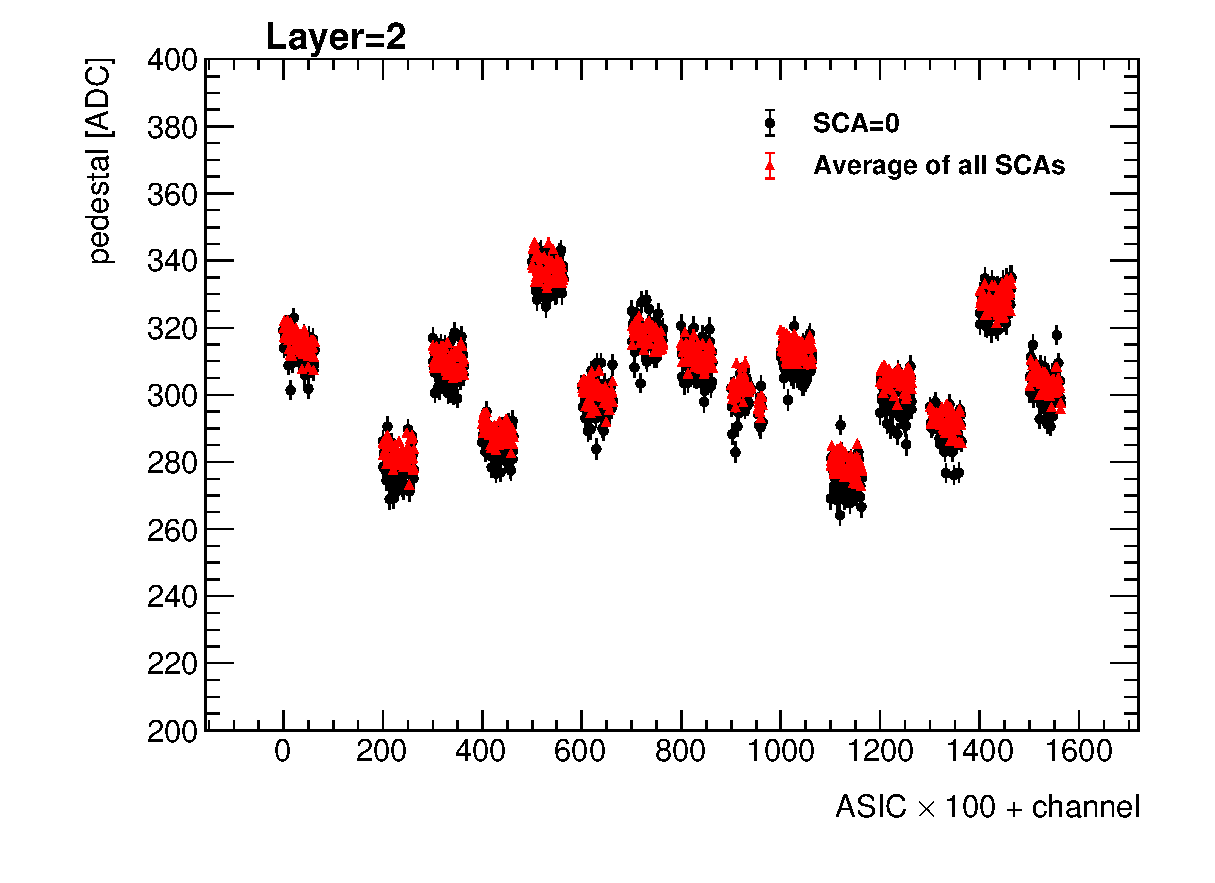
\includegraphics[width=2.8in]{figs/pedestal/ped_mean_layer2.eps} & 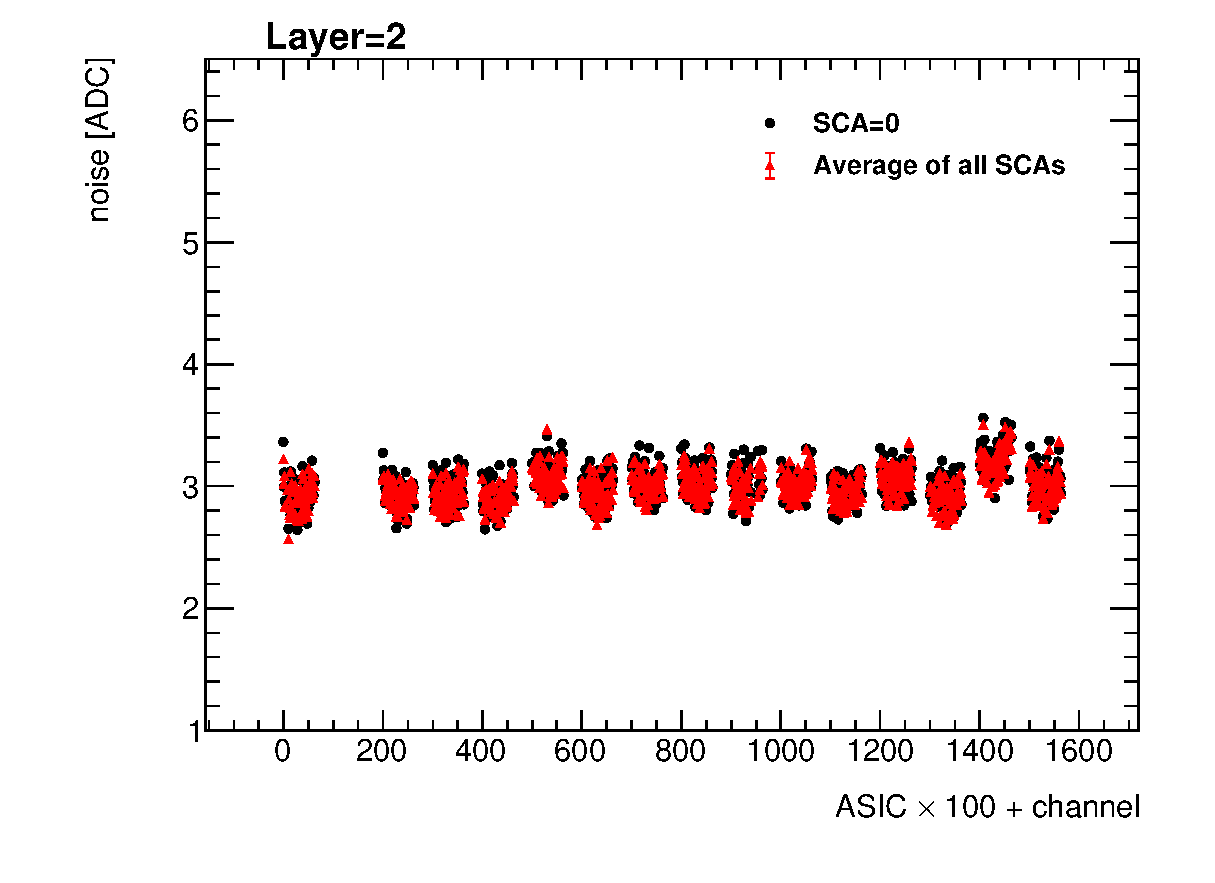
\includegraphics[width=2.8in]{figs/pedestal/width_mean_layer2.eps}
  \end{tabular}
  \caption{Pedestal mean position (upper plot) and width (lower plot) for all channels in one layer. The data is grouped on bunches in which the value in the x-axis
    corresponds to the value of the channel number plus the value of the ASIC number multiplied by 100. The black points show the value for the first SCA
    and the red points show the average value for all the others SCAs (with the standard deviation of the sample as error bar).}
\label{pedestal_layer}
\end{figure}

\begin{figure}[!t]
  \centering
  \begin{tabular}{ll}
    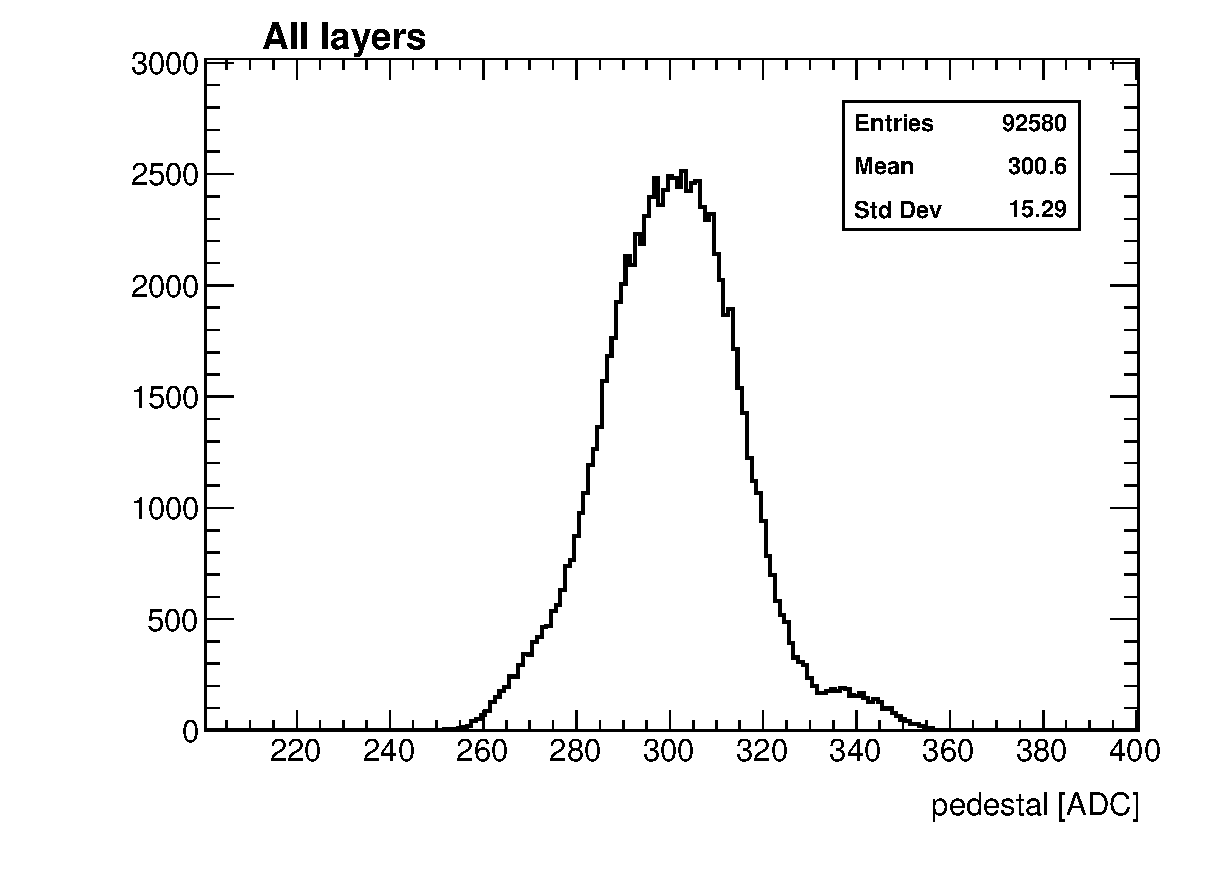
\includegraphics[width=2.8in]{figs/pedestal/h_ped_mean.eps} & 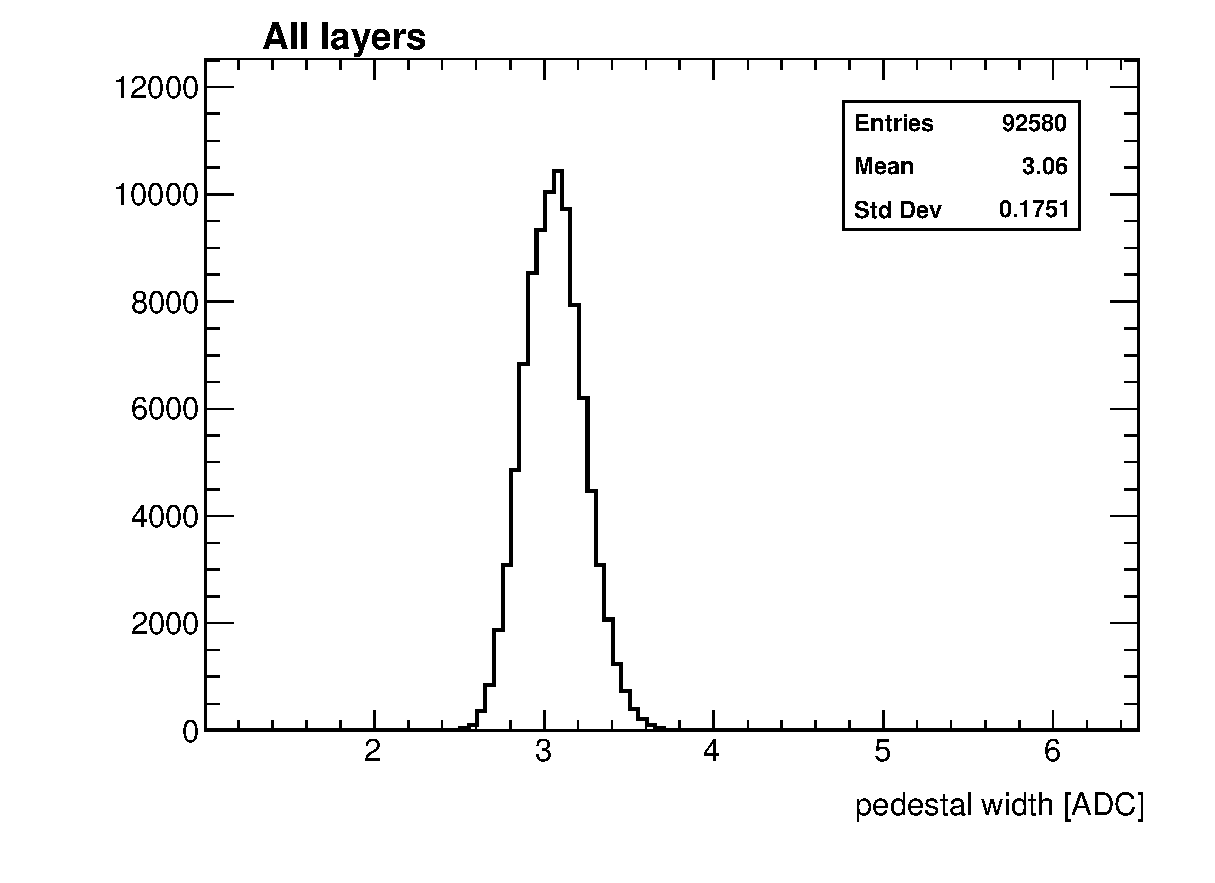
\includegraphics[width=2.8in]{figs/pedestal/h_ped_width.eps}
  \end{tabular}
  \caption{Pedestal mean position (left) and width (right) for all channels and all SCAs in the setup.}
\label{pedestal_all}
\end{figure}

\subsubsection{Energy calibration and tracking efficiency}
\label{sec:mip}

A Landau function convoluted with a Gaussian is fit to the resulting hit distribution. 
The most-probable-value of the convoluted function is taken as the MIP value, allowing thus for a direct
conversion from ADC units to energy in MIP units.
We have obtained a raw energy calibration spread of the 5\% among all channels with the 98\% of all 
available channels being fitted. Results are summarized in figure \ref{mipandSN}, leftmost plot.

\begin{figure}[!t]
  \centering
  \begin{tabular}{ll}
      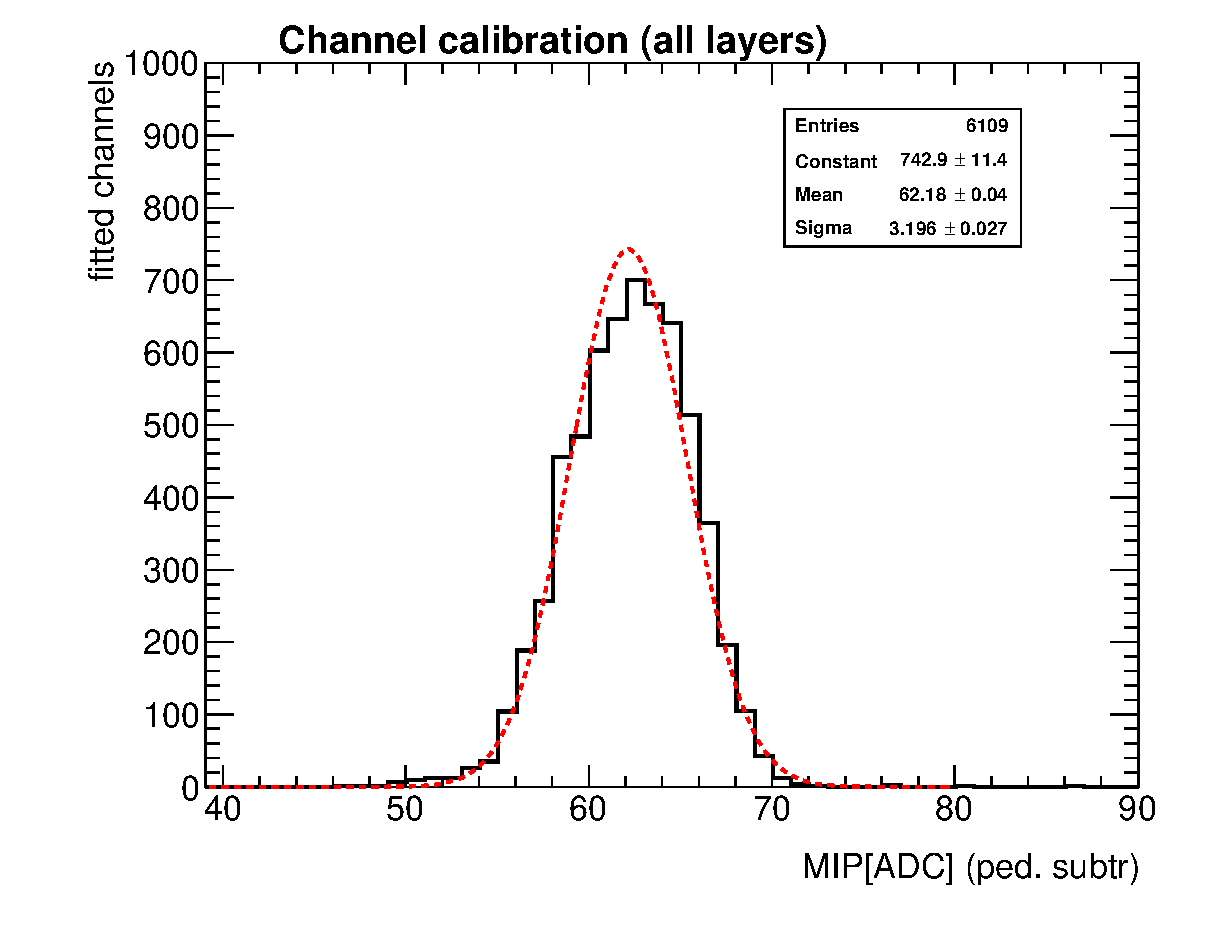
\includegraphics[width=2.8in]{figs/MIP/MIPsummary_title.eps} & 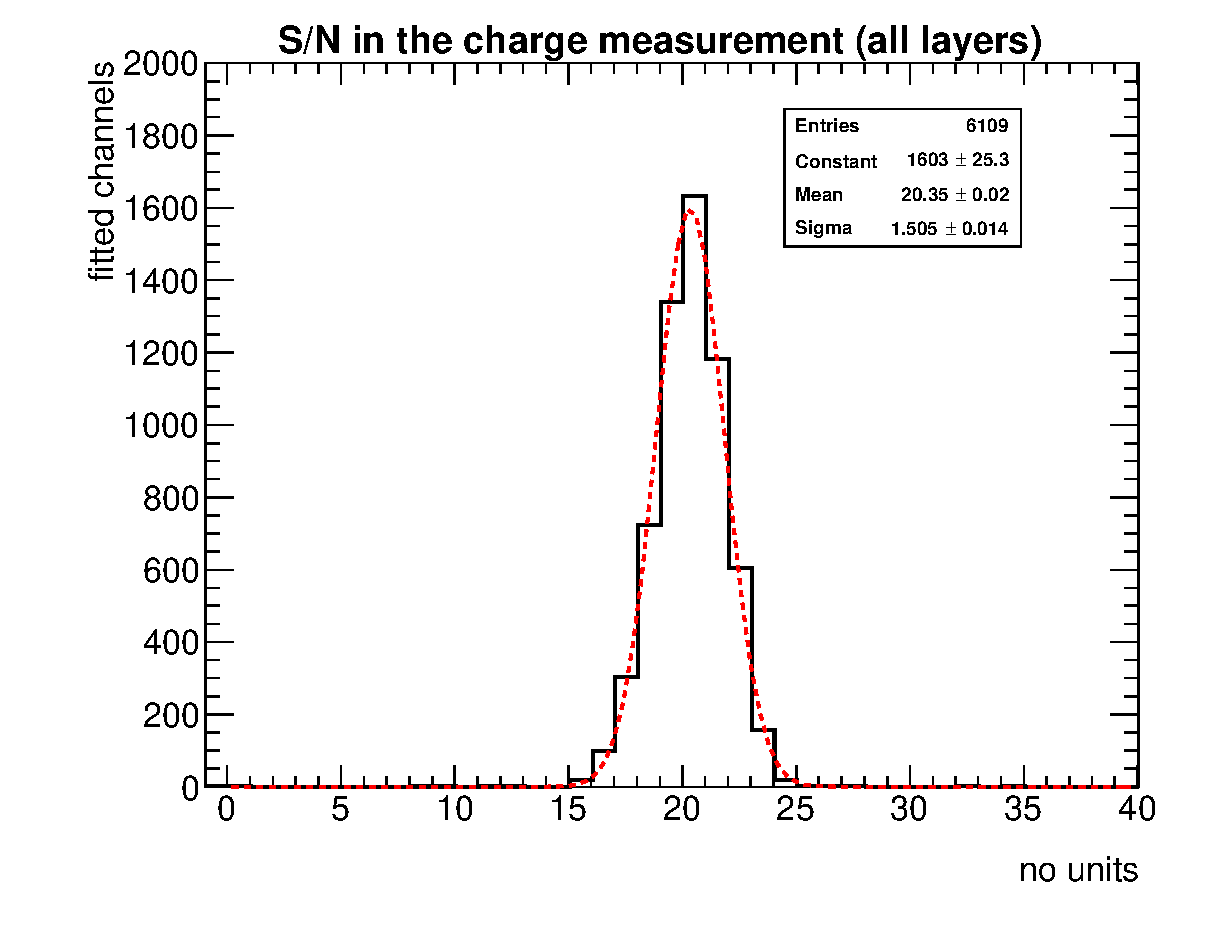
\includegraphics[width=2.8in]{figs/MIP/SNsummary_title.eps}  
  \end{tabular}
\caption{Result of the MIP position calculation and signal over noise calculation for all calibrated channels.}
\label{mipandSN}
\end{figure}

We checked the MIP 
calibration in all callibrated channels by selecting tracks
incident perpendicullary to the layers surface.
The results are shown in figure \ref{mip3peaks} where the single channel energy 
distribution for MIPs is shown for all calibrated channels in the same distribution. 
The maximum peaks at 1 MIP as expected after a good calibration.
In addition to this, a second and a third peak
appear visible. These peaks are due to
events involving multiple 
particles crossing the detector.

\begin{figure}[!t]
  \centering 
    \begin{tabular}{ll}
      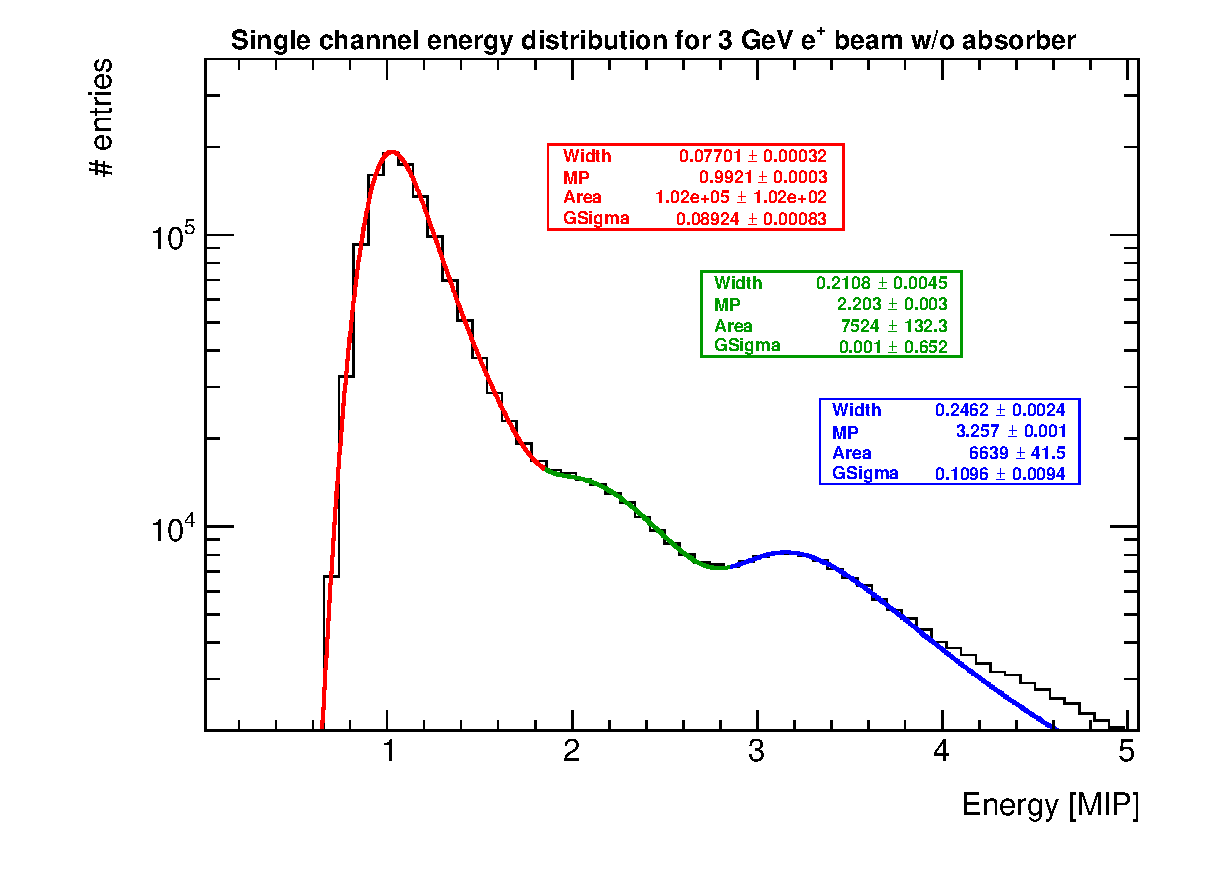
\includegraphics[width=4in]{figs/MIP/MIP3peaks.eps} 
    \end{tabular}
    \caption{Energy distribution for all callibrated channels when selecting tracks of 3 GeV positron acting as MIPs.}
\label{mip3peaks}
\end{figure}

To evaluate 
the single hit detection efficiency we define a high purity sample of
events by selecting
tracks with at least 4 layers with a hit in exactly the same channel. Afterwards we 
check if the other layers have or not a hit in the same channel (expanding the search
to the closest neighbouring channels) with energy larger or equal than 0.3 MIP.
Finally, we repeat this for all layers 
and channels. The results are shown in Figure \ref{efficiency}. Except few exceptions, the efficiency is 
compatible with $100\%$.
Lower efficiencies in the first layer are related to the presence of
noisy channels not spotted during the commissioning. In the last layer (separated from the
other layers by four slots of 1.5 cm instead of only one) we also observe few small deviations
from the $\sim100\%$ which are indeed
associated to a slight misalignment of the detector.
If we remove these channels from the analysis
the full efficiency is recovered.

\begin{figure}[!t]
  \centering 
    \begin{tabular}{ll}
      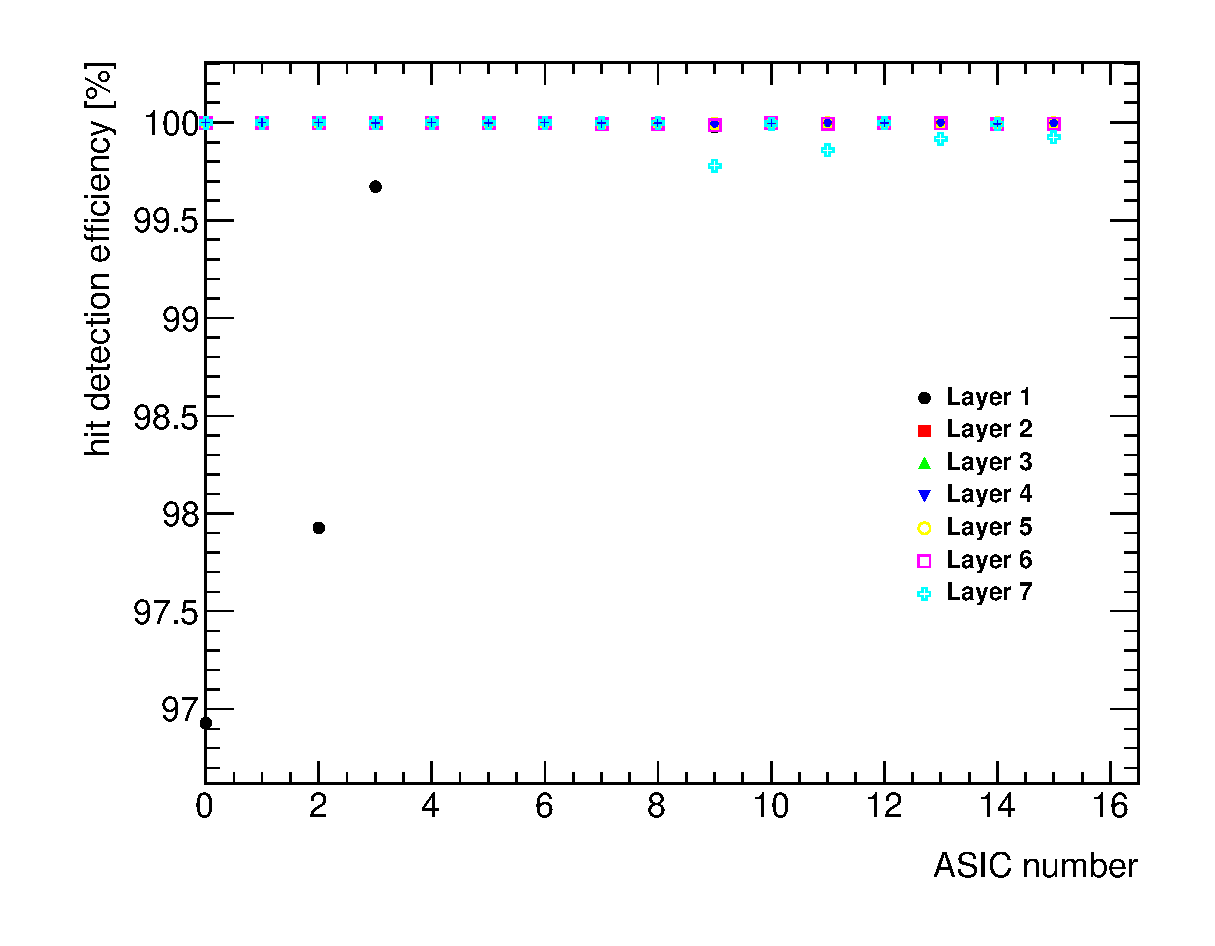
\includegraphics[width=2.8in]{figs/MIP/efficiency_nhits4_chips.eps} & 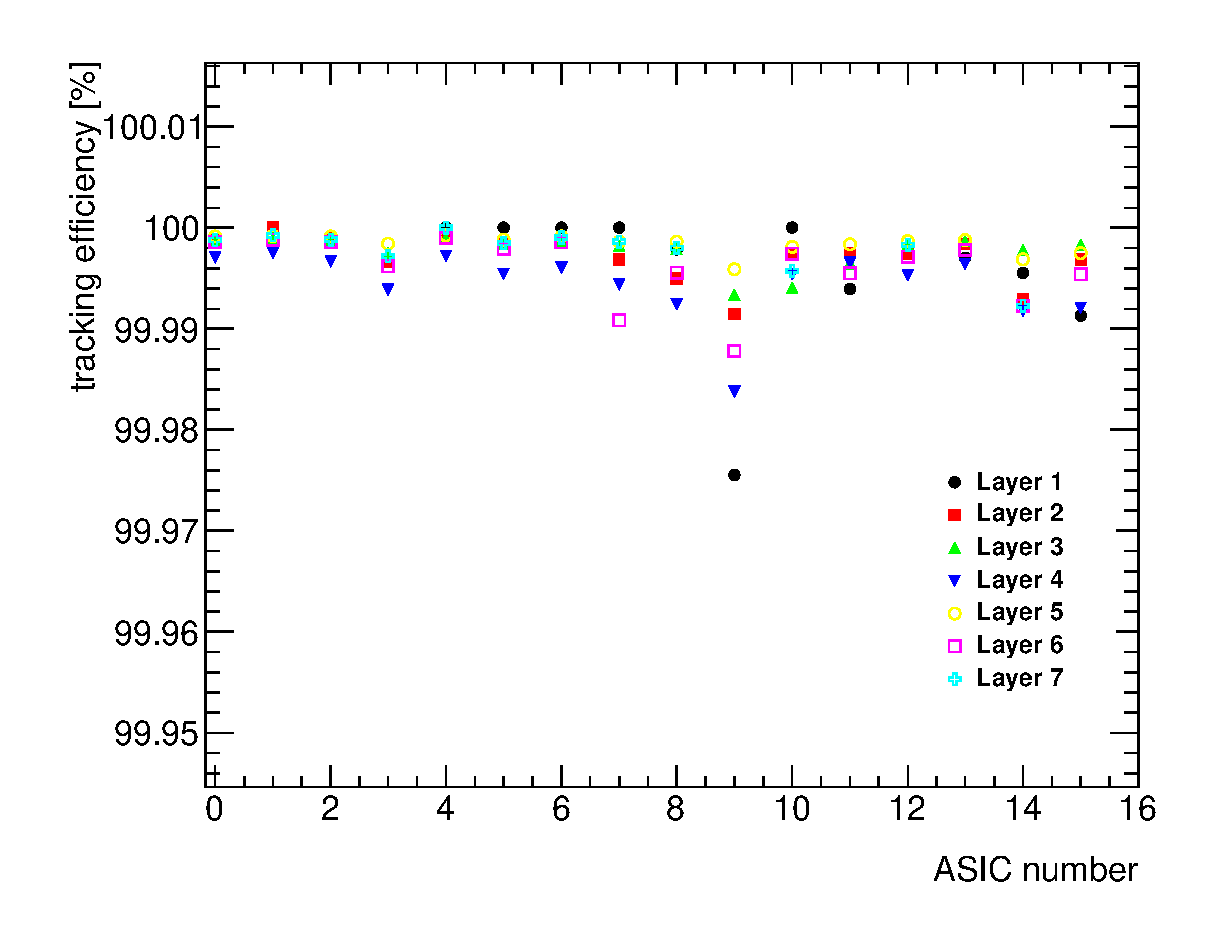
\includegraphics[width=2.8in]{figs/MIP/efficiency_nhits4_chips_zoom.eps} \\
    \end{tabular}
    \caption{Left: MIP detection efficiency for all layers and ASICs in high purity samples of tracks of MIP-like acting particles. Right: same figures with a zoom in the y-axis. In both cases, the average efficiency of the 64 channels in each ASIC is shown.}
\label{efficiency}
\end{figure}


\subsubsection{S/N ratio in the charge measurement for MIP interactions}
\label{sec:sn}

The signal-over-noise ratio in the charge measurement (corresponding to the slow shaper of the SKIROC2) is defined 
as the ratio between the most-probable-value of
the Landau-gauss function fit to the data (pedestal subtracted) and the noise (the pedestal width). This quantity 
has been calculated for all channels and all layers. The average S/N is to 20.4.
Results are summarized in Figure \ref{mipandSN}, rightmost plot.

\subsection{Pedestal and noise stability in a magnetic field}
\label{sec:magnetic}

The data taking inside the magnetic field has been divided in three steps:
a) a with a magnetic field of 1 T; b) a run with 0.5 T; c) a final run with the magnet off.
The beam, 3 GeV positrons, was hitting in the area of the PCB readout by the ASIC number 12.

The pedestal positions and noise levels of the channels of the ASIC 12 when the
SLAB is inside of the PCMag are compared with the results from the calibration run described in the previous section.
This is shown in Figure \ref{pedestal_magnetic}.
We see that the agreement is perfect within the statistical uncertainties.
Due to the lower rates in this beam area, the
analysis is only done up to few SCAs.

\begin{figure}[!t]
  \centering
  \begin{tabular}{ll}
    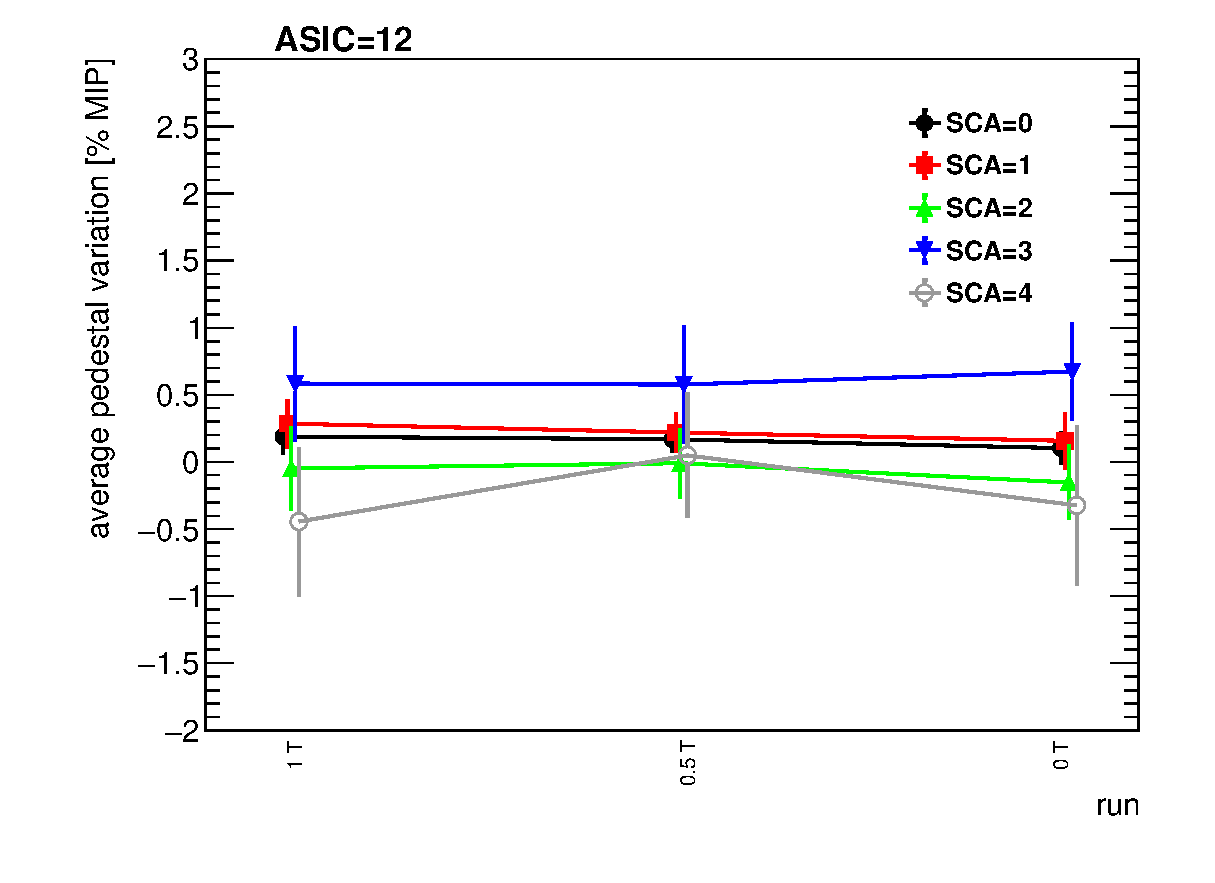
\includegraphics[width=2.8in]{figs/pedestal/1T/summary_pedestal_chip12.eps} & 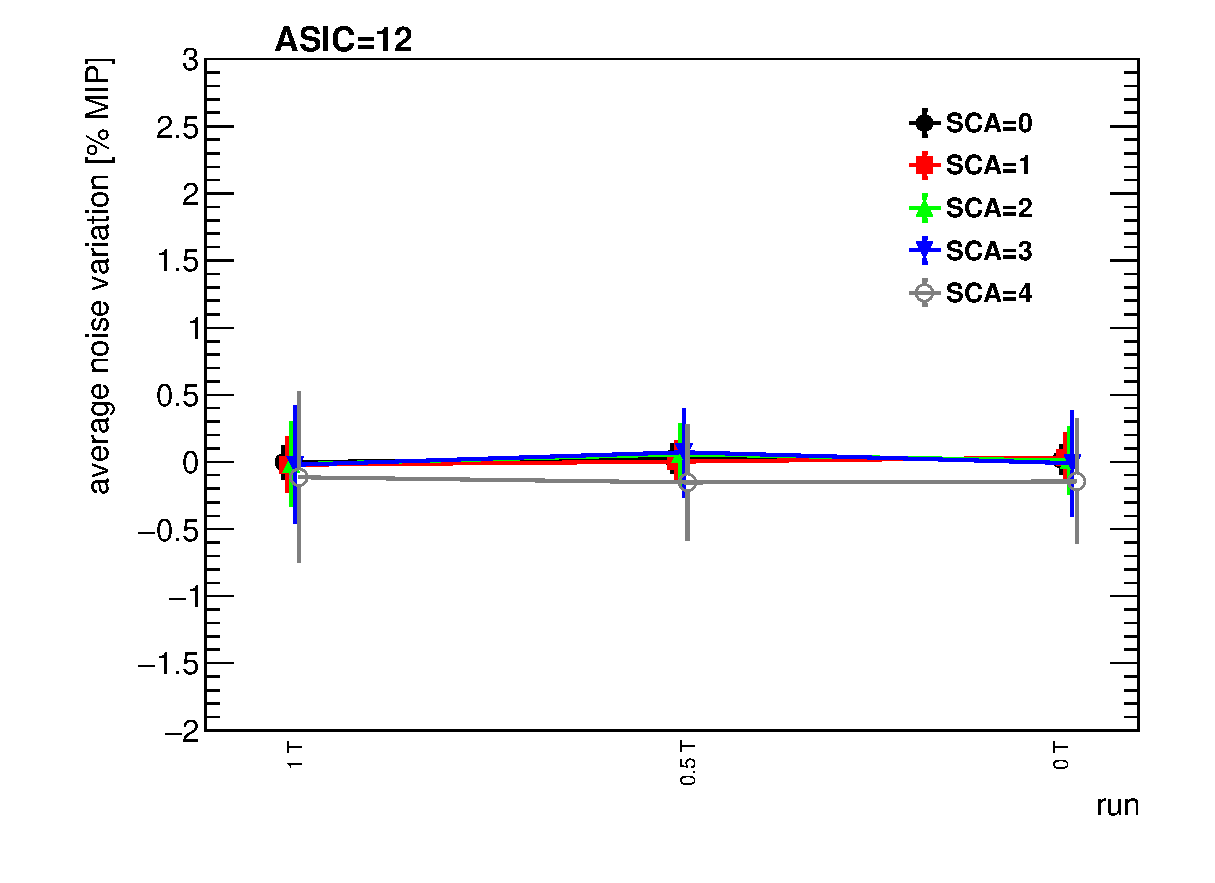
\includegraphics[width=2.8in]{figs/pedestal/1T/summary_noise_chip12.eps}
  \end{tabular}
  \caption{Average deviation of the pedestal mean position (left) and width (right) for all channels in the ASIC 12.}
\label{pedestal_magnetic}
\end{figure}

\subsection{Pedestal stability in electromagnetic shower events}
\label{sec:showers}

In this section we discuss the pedestal stability in events with large amount of charge collected by the ASICs, as are the 
electromagnetic shower events. All the results shown in this section correspond to data taken during the tungsten program, 
using the W-configuration number 2 when shooting the beam in the area registered by the ASIC 12 (and partially in the 13). 
Only information recorded by ASIC 12 is used in the analysis. For other configurations we get comparable results.
In order to select a high purity of
electromagnetic shower like the events, 
we used a simple criteria: select only events with at least 6 of the layers with at least a hit with E > 0.5 MIP.

\begin{figure}[!t]
  \centering 
    \begin{tabular}{ll}
      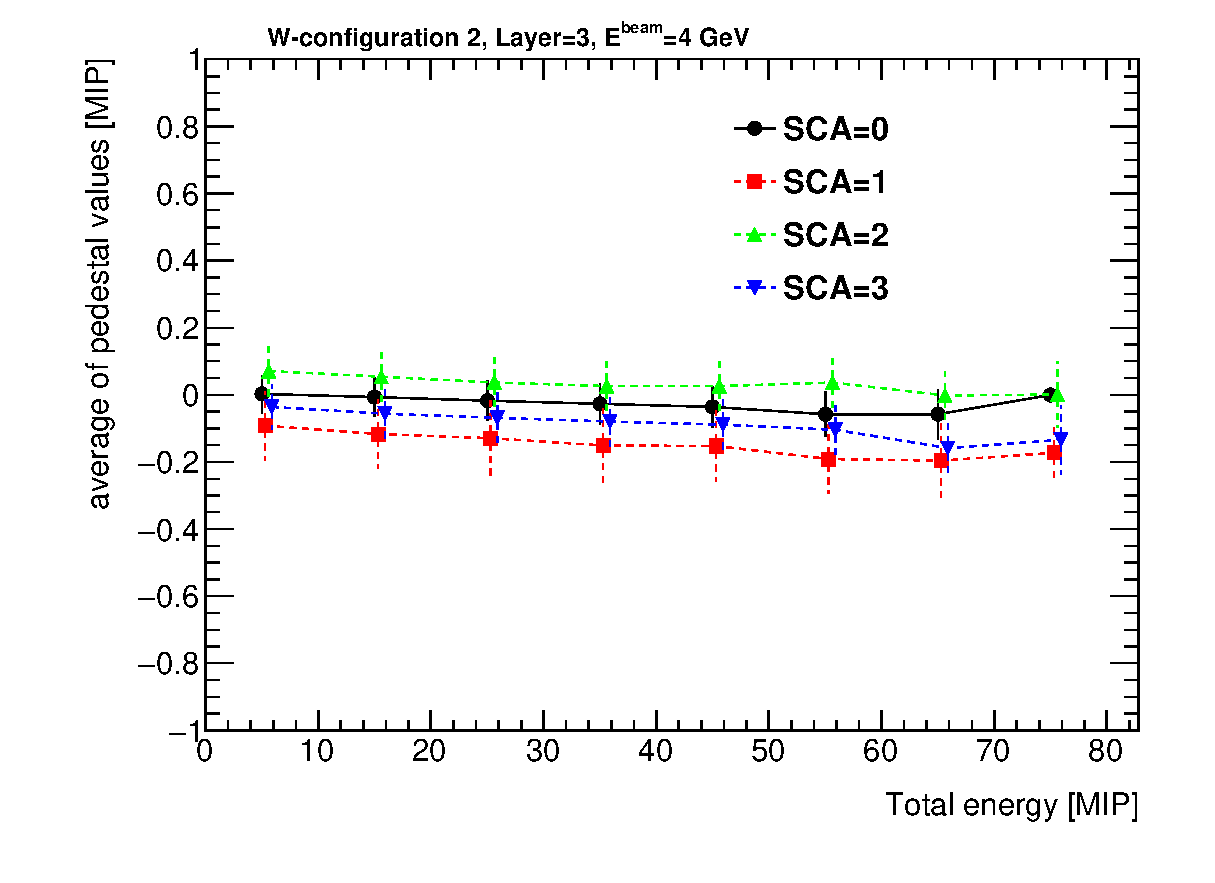
\includegraphics[width=2.8in]{figs/pedestal/pedestal_vs_energy_shower.eps} & 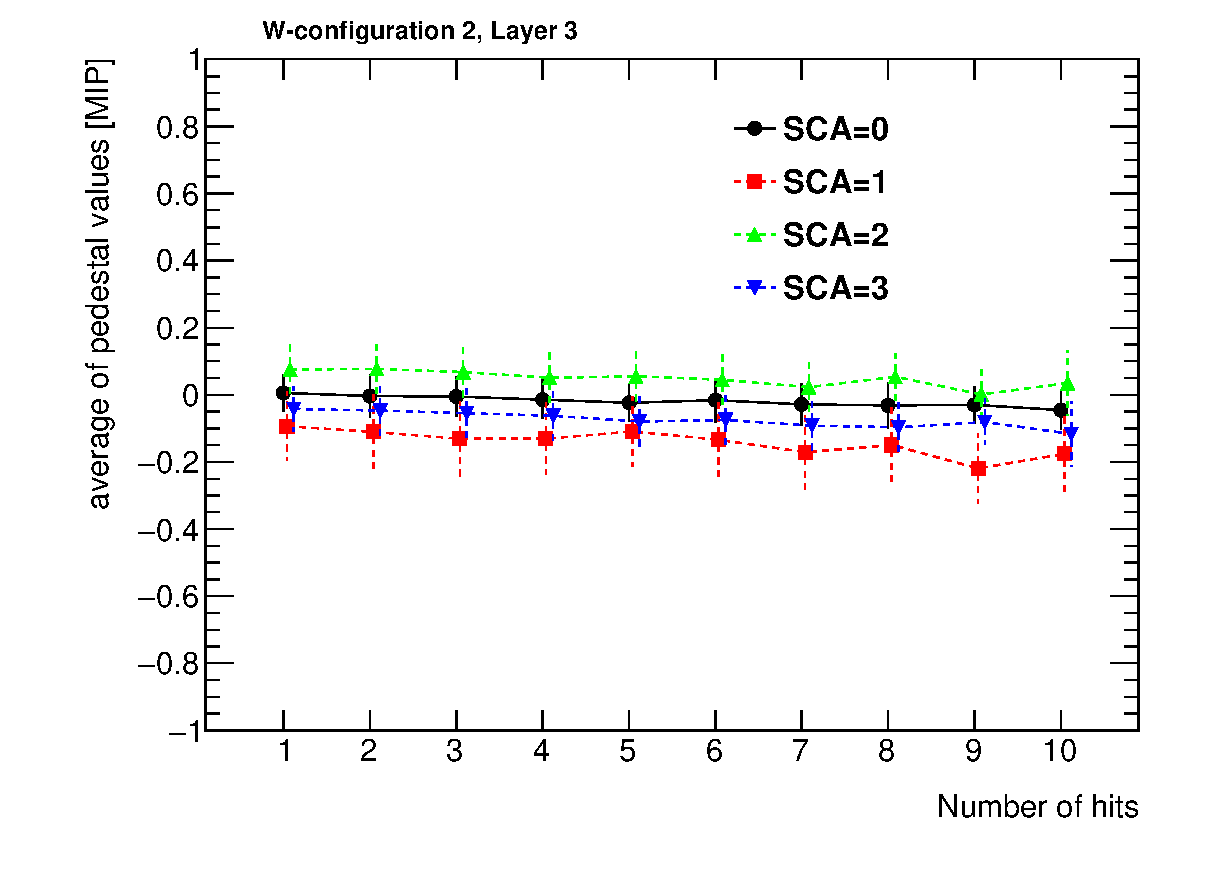
\includegraphics[width=2.8in]{figs/pedestal/pedestal_vs_nhits_shower.eps} \\
    \end{tabular}
    \caption{Left: mean position of the projection of the pedestal distribution of all channels
      calculated when different energies are collected in the ASIC (in bins of 10 MIPs).
      Right: same but as a function of the number of hits. In both cases, the results are shown for few SCA.
      The points for the curves with SCA larger than zero are slightly shifted in the x-axis to optimize the visualization.}
\label{pedestal_shower_1}
\end{figure}

Two main observations have been extracted from the recalculation of the pedestals and its comparison
with the values obtained previously during the calibration runs. The first observation
consists in a relatively small 
drift of the pedestal values
towards lower values when the collected energy is high (or when the number of triggered channels is large).
%For events with 80 MIPs collected in the ASIC, we have an average drift of the pedestal of $\sim$ 0.05 MIP. 
This is shown in Figure \ref{pedestal_shower_1} for several SCAs where the
average of the projection of the pedestal distribution for all channels non triggered in ASIC 12 of layer 3 
is plot as a function of the total energy measured by the ASIC (or the total number of hits).
We see that in both cases, the shapes of the curves 
for each SCA are very similar.
This feature is known and it is due to the architecture of the SKIROC2 ASICs 
where high inrush of currents can slightly shift the baseline of the analogue power supply. 
%This feature is foreseen to be removed from the SKIROC3 ASICs. 

The second observation extracted from this analysis can be also seen in Figure \ref{pedestal_shower_1} but
more clearly in Figure \ref{pedestal_shower_2}: in addition
to the small drift of the pedestal value an SCA-alternate global shift
is observed. We see that the effect is enhanced when large amounts of charge
are deposited in the ASIC ({\it i.e.} at larger beam energies or for the layers in the maximum of the shower
profile). We also observed that this alternation is only SCA dependent and does not depends
on the time in which the deposit of energy occurs within the acquisition.
This is not yet fully understood although the fact that the effect is observed in
alternate SCAs hints that something is affecting to the digital part of the ASIC 
(where the SCAs enter in play).
Dedicated tests in the laboratory and in the beam are needed in order to clarify this issue.

\begin{figure}[!t]
  \centering 
    \begin{tabular}{ll}
      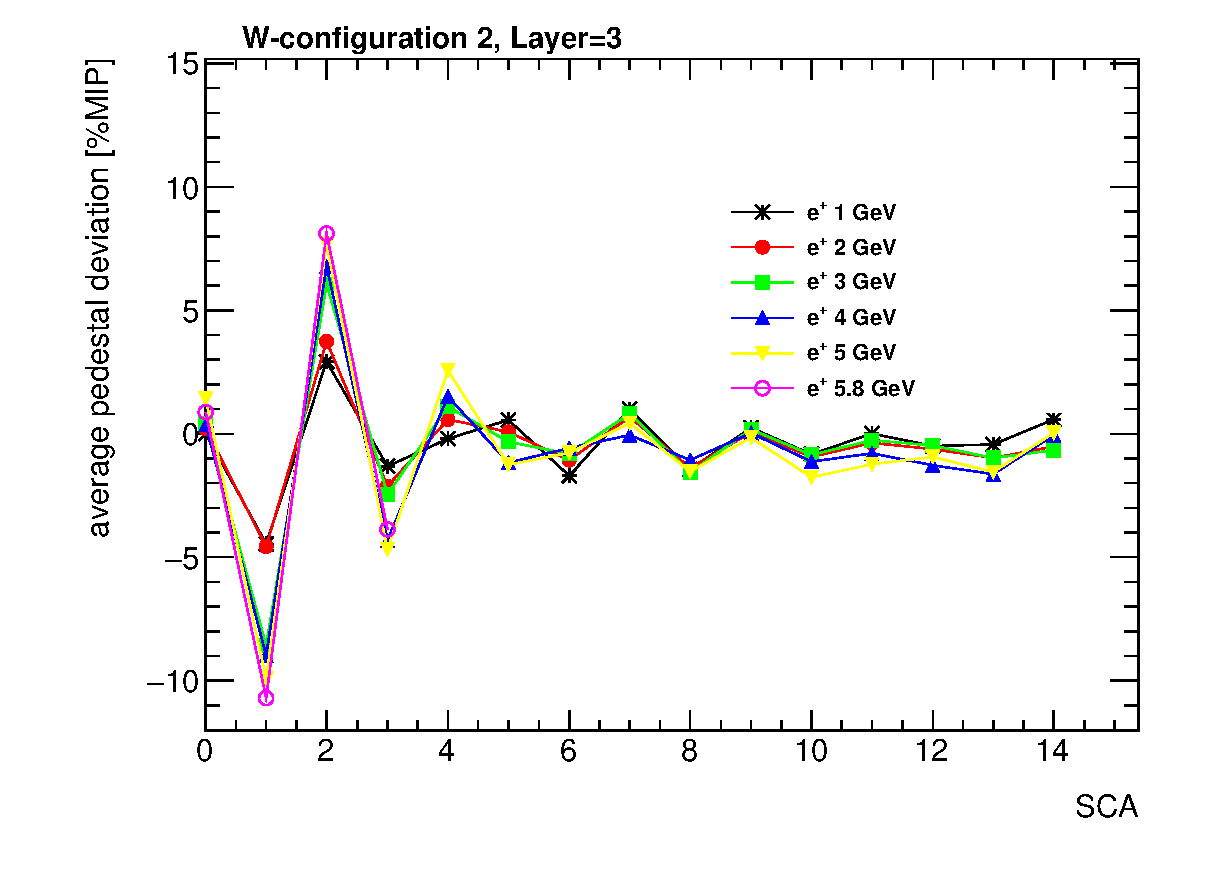
\includegraphics[width=2.8in]{figs/pedestal/pedestal_deviation_layer3.eps} & 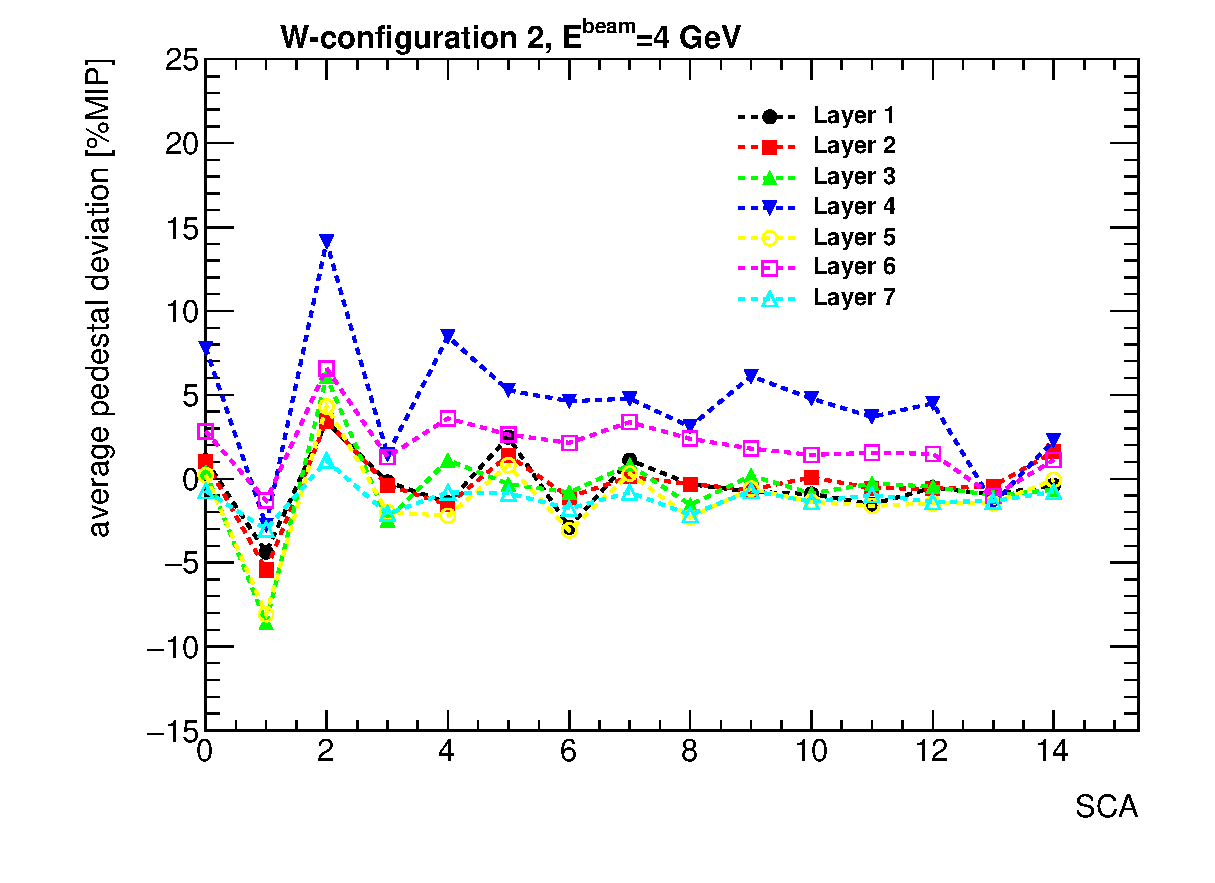
\includegraphics[width=2.8in]{figs/pedestal/pedestal_deviation_4GeV.eps} \\
    \end{tabular}
    \caption{Left: average value on each SCA of the calculated pedestals for all channels of ASIC 12 in the Layer 3 for different energies of the beam. Right: same but fixing the energy of the beam and comparing several layers.}
\label{pedestal_shower_2}
\end{figure}


\section{Summary}
\label{sec:summary}

The R\&D program of the highly granular SiW-ECAL detector is in an exciting phase. 
After the proof of principle of the imaging calorimetry concept using the physics prototype, the 
technological prototype is being constructed and tested. In this document we describe the commissioning and
beam test performance of a prototype built in with the first fully assembled
detector elements.

A very comprehensive and detailed commissioning procedure has been established and optimized
allowing us to identify and isolate the different noise sources that could spoil the data taking.
The beam test has provided a lot of useful data to study 
the performance of the detector and  to perform
a channel by channel calibration.
A full analysis of the MIP calibration within magnetic field and
the response of the prototype in electromagnetic shower events
will be covered in a future document.
In addition, the results shown here serve as input
for ongoing and future R\&D.

\section{Outlook}
\label{sec:outlook}

In parallel to the work described here, several R\&D efforts are being carried.
One of these efforts is directed to the design and test of new ASICs.
In fact, a new generation of SKIROC2, the 2a, has been delivered
and it is being tested in the dedicated testboards and it has been integrated in new ASUs.
In addition, a new generation of the ASIC, SKIROC3, is foreseen for the final detector construction.
In contrast with SKIROC2/2a, the new ASIC will be fully optimized for ILC operaton, {\it i.e.} full zero suppression, reduced power consumption etc.

Many efforts are also concentrated in the construction and test of long SLABs
made of several ASUs enchained since we know that the ILD ECAL will host long layers of up to $\sim$2.5m.
This device constitutes a technological challenge in both aspects, the mechanical
(very thin and long structure with fragile sensors in the bottom, complicated assembly procedure...)
and the electrical (i.e. transmission of signals and high currents).
For example, interconnections between ASUs and between ASU and interface card are one of
the most involved parts of the assembly
and require close collaboration between mechanical and electronic engineers.
The construction and test of a long SLAB prototype
of $\sim8$ ASUs is currently ongoing.
%Therefore, many efforts are focused in the construction and test of such long 
%layers made of chains of ASUs (up to $\sim$15 ASU) 
%as well as in the standardization of the interconnections. 

In parallel to the ASUs equipped with BGA packaged ASICs, a different proposal for the ASU
design is being investigated. This is motivated by the high density of channels
demanded by the Particle Flow algorithms. Indeed, the FEV11 thickness is 1.6 alone and 2.7 mm
including the ASICs in its current packaging: 1.1 mm thick LFBGA package.
In this alternative PCB design the ASICs
are directly placed on board of the PCB in dedicated cavities.
The ASICS will be in semiconductor packaging and wire bonded to the PCB. This is the so-called COB (chip-on-board) version of the ASU.
A small sample of FEV11\_COBs (same connexion pattern with the interface card than FEV11)
with a total thickness of 1.2 mm allowing for a potential denisty of 10000 channels/dm$^{3}$ has been produced and tested in the laboratory
showing its readiness for tests with particle beams. A sample can be seen in Figure \ref{cob}.

\begin{figure}[!t]
  \centering
    \includegraphics[width=2.8in]{figs/fev11_cob.png} 
  \caption{Two FEV11\_COB boards with 16 SKIROC2a wire bonded. The ASICs are protected with watch glasses.}
\label{cob}
\end{figure}

Finally, many efforts in the compactification of
the DAQ and the ASUs ({\it i.e.} the chip on board versions of the 
ASUs described in Section \ref{sec:ASU}) are being
conducted by the SiW-ECAL collaboration.

It is foreseen that all these developments, with the exception of the SKIROC3, will be tested with particle beams during 2018-2019.


\acknowledgments

This project has received funding from the European Union{\textquotesingle}s Horizon 2020 Research and Innovation program under Grant Agreement no. 654168.
This work was supported by the P2IO LabEx (ANR-10-LABX-0038), excellence project HIGHTEC,
in the framework {\textquotesingle}Investissements d{\textquotesingle}Avenir{\textquotesingle}
(ANR-11-IDEX-0003-01) managed by the French National Research Agency (ANR).
The research leading to these results has received funding from the People Programme (Marie
Curie Actions) of the European Union{\textquotesingle}s Seventh Framework Programme (FP7/2007-2013)
under REA grant agreement, PCOFUND-GA-2013-609102, through the PRESTIGE
programme coordinated by Campus France.
The measurements leading to these results have been performed at the Test Beam Facility at DESY Hamburg (Germany), a member of the Helmholtz Association (HGF).

\appendix
\section{Apendix: Filtering of fake triggers}
\label{sec:retriggers}

Several types of fake signals have been observed in the technollogical prototype since its construction and test. A detailed description of them
can be found in previous articles, as for example, in Ref. \cite{Amjad:2014tha}. All these fake signals are easily identified
and tagged during the data acquisition and removed afterwards from the analysis
not introducing any significance loss of performance as can be seen, for example, in the hit detection efficiency plots (see Section \ref{sec:mip}).
In the following, we briefly describe the status of the monitoring, debugging and filtering
of such kind of events.

\subsubsection*{Empty triggers}

Empty trigger events are a well known feature of SKIROC2. The SKIROC2 uses
an OR64 signal to mark the the change to a new SCA when a signal over threshold is
detected. The empty triggers appear when during
the acquisition the rising edge of the slow clock falls during the OR64 signal
and therefore the change to a new SCA is validated twice.
This effect creates around 10-15\% of empty events which are easily filter and removed from the
analysis. \todo{The ratio of empty triggers in the new SKIROC2a is reduced to the $\sim3\%$
thanks to to a decrease of the OR64 size by a factor X.}

\subsubsection*{Plane events and retriggers}

Another well know issue is the appearance of bunches of consecutive fake triggers, called retriggers,
that saturates the DAQ. These events are also
characterized by triggering many channels (some times even all channels of an ASIC) at the same time.
Although the ultimate reason of the appearance of these events remains unknown we
think that they may be related to some distortion of the
power supply baselines. We know that the SKIROC2 and 2a preamplifiers are referenced to the analog power supply level,
therefore, any voltage dip can ve seen as signal by the preamplifiers. The presence of a high inrush of current
due to many channels triggered at the same time can create these voltage dips
and produce the so called plane events (most of the channels trigered at once).
In previous studies ({\it i.e.} reference \cite{Amjad:2014tha}), the ratio of retriggers and plane events
was reduced by improving the power supply stabilization capacitances. It is important to remark that
all layers and all ASICs analog and digital levels are powered using the same power supply.
Moreover, the high voltage power supply for the polarization of the PIN diode it is also common for all layers.
Therefore any noise in
these power supplies or any overload of an ASIC may participate in the creation of fake signals
in different ASICs and layers.

Studying the MIP calibration data of this beam test we have noticed that the larger concentration of the retriggers and plane events are originated 
in
ASICs far from the beam spot. Even more, hot spots tend to appear near the channels 37 and the channels masked
as suspicious of suffering from routing issues. The amount these events have been estimated to be of $1-3\%$ in the ASICs where high frequency
interactions are produced ({\it i.e.} using 3 GeV positrons ate 2-3 KHz) and at higher rates even larger than $40\%$ in other 
ASICs far from the beam spot.
Moreover, it has been noticed a correlation between the time that an ASIC was full and the time of the appearance of some 
retriggers in other areas of the PCB. 
This correlation corresponds to $\sim$1.6 $\mu$s which hints
of a distortion on the analogue power supply when
the signal that informs the DIF that one ASIC memory is full is transmitted through the PCB.

All this information and dedicated studies in the laboratory will be used for the
improvement of the power supplying system, the PCB design and for further SKIROC developments 
with the possible approval the ILC in the scope.

% We suggest to always provide author, title and journal data:
% in short all the informations that clearly identify a document.

\bibliographystyle{JHEP}
\bibliography{references}

\end{document}
